%####################################################################
%############ BEGIN PREAMBLE ########################################
%####################################################################
\documentclass[12pt]{report}

%Packages-------------------------------------
\usepackage{amsmath}
\usepackage{amsfonts}
\usepackage{amssymb}
\usepackage{amsthm}
\usepackage{graphics}
\usepackage{graphicx}
\usepackage{subfigure}
\usepackage{relsize}
\usepackage{tabularx}
\usepackage{multirow}
\usepackage[nopostdot,style=list,nonumberlist,toc]{glossaries}
%\usepackage{hyperref}
\usepackage{xurl}
\usepackage[nottoc]{tocbibind}
\usepackage{caption}
\usepackage{float}
\usepackage{setspace}

%\usepackage{xtocnic}

\usepackage[localise=on]{xepersian}

\settextfont[Scale=1]{XB Zar}
%\setdigitfont[Scale=1]{XB Zar}
\setlatintextfont[Scale=1]{Times New Roman}

%Layout---------------------------------------

%\usepackage[top=2cm, bottom=2cm, left=2cm, right=2cm]{geometry}

%Commands-------------------------------------
\setcounter{tocdepth}{3}
\setcounter{secnumdepth}{3}
\renewcommand{\arraystretch}{1.25}

%Theorems-------------------------------------
\newtheorem{thm}{قضیه}[chapter]
\newtheorem{cor}[thm]{نتیجه}
\newtheorem{defn}[thm]{تعریف}
\newtheorem{prop}[thm]{گزاره}
\newtheorem{lmm}[thm]{لم}
\newtheorem{conj}[thm]{حدس}
\newtheorem{exm}[thm]{مثال}
\newtheorem{rem}[thm]{تذکر}
\newtheorem{note}[thm]{یادداشت}
\newtheorem{alg}[thm]{الگوریتم}


%Glossaries-----------------------------------
\makeglossaries
\loadglsentries{glossaries}

%Folder of Figures----------------------------
\graphicspath{{./figures/}}
%####################################################################
%########### END PREAMBLE ###########################################
%####################################################################


%####################################################################
%########### BEGIN DOCUMENT #########################################
%####################################################################
\begin{document}
	
	%Title page ----------------------------------
	
	\begin{figure}
		\centering
		
\includegraphics[height=2.5cm]{ut.png}
	\end{figure}
	
	\begin{center}
		پردیس علوم
		\\
		دانشکده ریاضی، آمار و علوم کامپیوتر
	\end{center}
	
	\begin{center}
		%%%%%%%%%%%%%
	\end{center}
	
	\begin{center}
		\huge{مدل‌سازی سازوکارهای مسئله‌ی انقیاد در شبکه‌های عصبی ضربه‌ای}
	\end{center}
	
	\begin{center}
		%%%
	\end{center}
	
	\begin{center}
		نگارنده
	\end{center}
	\begin{center}
		\textbf{
			امیر اصلان اصلانی
			\\[30pt]
		}
	\end{center}
	
	\begin{center}
		اساتید راهنما
	\end{center}
	\begin{center}
		\textbf{
			محمد گنج‌ تابش 
			\\[5pt]
			عباس نوذری دالینی
		}
	\end{center}
	
	\vspace{3cm}
	\begin{center}
		پایان‌نامه برای دریافت درجه‌ی کارشناسی ارشد
		\\
		در رشته علوم کامپیوتر
	\end{center}
	
	\begin{center}
		بهمن ۱۴۰۱
	\end{center}
	
	\pagestyle{empty}
	\pagenumbering{}
	
	\newpage
	%\pagestyle{headings}
	%\setcounter{page}{1}
	%\pagenumbering{roman}
	\pagestyle{plain}
	\setcounter{page}{1}
	\pagenumbering{harfi}
	
	%Abstract page-------------------------------
	
	\chapter*{}
	\section*{چکیده}
	مسئله‌ی انقیاد یکی از مسائل مهم در علوم اعصاب، علوم‌شناختی و فلسفه‌ی ذهن است که درباره‌ی چگونگی یکپاره شدن درک موجود زنده از محیط از مفاهیم جزئی تشکیل شده در مغز است. اهمیت این مسئله در درک کردن عملکرد‌‌های شناختی انسان است که خود بخشی از مراحل مورد نیاز برای طراحی سیستم‌هایی است که قادر به پردازش عملکرد‌های شناختی مشابه انسان هستند. تحقیقات نشان‌دهنده‌ی نقش بسیار پررنگ ستون‌های کورتکسی، که ساختار‌هایی در نئوکورتکس هسند، در عملکرد‌های شناختی موجودات زنده هستند. در این پژوهش تلاش شده تا با مدل‌سازی ستون‌های کورتکسی و روابط بین آن‌ها با استفاده از شبکه‌های عصبی ضربه‌ای، تشکیل انقیاد در مغز شبیه‌سازی شود. نهایتا آزمایش‌ها و بررسی‌های صورت گرفته روی مدل طراحی شده، به درستی شکل‌گیری انقیاد را نشان می‌دهند. این موضوع نشان‌دهنده‌ی این است که احتمالا ستون‌های کورتکسی، به عنوان ساختار‌هایی ثابت که در مدل‌سازی به سادگی قابل تکرار هستند، بالقوه ساختار‌های مناسبی برای استفاده در مدل‌سازی‌ها هستند و امکان شکل‌ گرفتن پردازش‌های شناختی را در مدل افزایش می‌دهند. 
	
	\section*{}
	\textbf{کلمات کلیدی:}\quad ستون کورتکسی، مسئله‌ی انقیاد، شبکه‌ی عصبی ضربه‌ای، مدل‌سازی.
	
	%Dedication page-----------------------------
	
	%\chapter*{تقدیم به}
	%\section*{تقدیم به}
	
	%Acknowledgement page------------------------
	
	%\chapter*{سپاسگزاری}
	%\begin{center}
	%    content...
	%\end{center}
	%
	%%copyright + declaration page
	%\chapter*{اصالت اثر}
	%\section*{اصالت اثر}
	% هیچ قسمت از این پایان‌نامه، پیش از این در هیج موسسه تحصیلات عالی برای دریافت درجه تحصیلی استفاده نشده است. همچنین، هیچ قسمت از این پایان‌نامه برگردان فارسی تمامی یا قسمتی از یک اثر دیگر علمی (مانند مقاله، پایان‌نامه، و غیره) به زبانی دیگر نمی‌باشد. ارائه این پایان‌نامه توسط نگارنده به معاونت آموزشی (معاونت پژوهشی و تحصیلات تکمیلی برای ارشد و دکتری) به منزله تعهد نگارنده به اصالت متن و محتوای ارائه شده بر اساس یک کار پژوهشی در مدت تحصیل در دانشگاه تهران می باشد. در صورت اثبات خلاف این امر، مدرک تحصیلی اخذ شده توسط این پایان‌نامه از دانشگاه تهران، معتبر نمی باشد.
	%
	%\chapter*{حق مالکیت معنوی}
	%\section*{حق مالکیت معنوی}
	%حق مالکیت معنوی این اثر متعلق به دانشگاه تهران می باشد. استفاده از مطالب این پایان‌نامه در فعالیت های تحقیقاتی با ذکر منبع بلامانع می‌باشد. در صورت استفاده تجاری، مانند چاپ این پایان‌نامه، هماهنگی لازم و اجازه کتبی از دانشگاه و نگارنده پایان‌نامه الزامی می‌باشد.
	%
	
	%-------------------------
	%\pagestyle{plain}
	%\setcounter{page}{1}
	%\pagenumbering{harfi}
	%-------------------------
	\onehalfspacing
	%Preface--------------------------------------
	
	\chapter*{پیشگفتار }
	برای مدت زمان بسیاری چگونگی کارکرد مغز انسان یکی از سوالات بشر بوده است و در دهه‌های اخیر، با پیشرفت فناوری، دانش ما از ساختار مغز بسیار افزایش یافته‌ است؛ اما همچنان چگونگی رخ دادن بسیاری از عملکرد‌های شناختی در موجودات زنده، یکی از اصلی ترین پرسش‌های پژوهشگران است. افزایش دانش ما از ساختار مغز با پیدایش سیستم‌های محاسبه‌گر و پس از آن با افزایش قدرت محاسباتی همراه بوده که از طرفی موجب پیشرفت‌های بسیار چشم‌گیری در حوزه‌ی هوش مصنوعی شده. کنجکاوی بشر در چگونگی عملکرد مغز انسان از یک سو و پیش‌رفت‌های هوش مصنوعی از سوی دیگر باعث شده تا بسیاری از پژوهشگران با تلاش برای مدل‌سازی فعالیت‌های مغزی به سمت تولید سیستم‌های هوشمند با عملکرد‌های شناختی مشابه انسان گام بردارند. در این میان علوم‌اعصاب محاسباتی به عنوان یک حوزه‌ی بین رشته‌ای، که از طرفی با علوم اعصاب در ارتباط است و از طرف دیگر با علم کامپیوتر، در سال‌های اخیر پیش‌رفت‌های بسیاری داشته که موجب شده تا بسیاری از محققان به پژوهش در این حوزه رو آورند.
	
	یکی از موضوعات اساسی که چگونگی رخ دادن آن در موجودات زنده همچنان به صورت واضح مشخص نشده است مسئله‌ی انقیاد است. موجودات زنده محیط خود را از طریق درون‌داد‌های عصبی خود همچون بینایی، شنوایی و لامسه احساس می‌کنند و تک تک اجزای اطلاعات دریافت شده به صورت مجزا و تفکیک شده در مغز شکل می‌گیرند؛ ولی نهایتا موجود زنده به یک درک یکپاره از مفاهیم اطراف خود می‌رسد. برای مثال در مغز فردی که تصویر یک مربع مشکی که با رنگ قرمز پر شده است را می‌بیند به صورت مجزا مفهوم چهار خط مشکی و رنگ زرد شکل می‌گیرد ولی در پردازش‌های شناختی نهایتا این مفاهیم جدا از هم به صورت یک مفهوم واحد تجمیع می‌شوند و یک مربع با رنگ قرمز را در ذهن فرد تداعی می‌کنند.
	
	پدیده‌ی انقیاد به عنوان یکی از مهم‌ترین ویژگی‌های شناختی انسان مورد توجه بسیاری از پژوهشگران قرار گرفته و در عصر امروز که هوش مصنوعی و به خصوص شبکه‌های عصبی مصنوعی با سرعت بسیاری در حال پیش‌رفت هستند عدم امکان رخ دادن انقیاد در آن‌ها به عنوان یکی از محدودیت‌های اصلی آن‌ها بیان می‌شود و به همین دلیل تلاش‌های بسیاری برای پیاده‌سازی سازوکار‌هایی برای وارد کردن انقیاد به شبکه‌های عصبی مصنوعی در حال انجام است. شبکه‌های عصبی مصنوعی ضربه‌ای به عنوان نسل سوم شبکه‌های عصبی مصنوعی و یک مدل بسیار زیست‌توجیه پذیر یک ابزار بسیار مناسب برای مدل‌سازی مدلی است که انقیاد در آن قابل مشاهده باشد. به همین منظور، در این مطالعه مدلی زیست توجیه‌پذیر با استفاده از شبکه‌های عصبی ضربه‌ای و با الهام از ساختار‌هایی به نام ستون‌های کورتکسی در مغز پیاده‌سازی شده است که در تلاش است تا سازوکار انقیاد را به صورت رایانشی مدل‌سازی کند.
	
	این پایان‌نامه در پنج فصل به صورت زیر تنظیم شده است:
	
در فصل اول، برخی از مفاهیم اولیه‌ی مرتبط با سیستم عصبی انسان، مسئله‌ی انقیاد و شبکه‌های عصبی ضربه‌ای را به صورت مختصر مرور خواهیم کرد.

در فصل دوم با بیان مسئله‌ی کلی مورد نظر و مشکلات حال حاضر در آن موضوع، به طرح کردن مسئله‌ای که قصد پاسخ به آن را داریم خواهیم پرداخت.

در فصل سوم به برخی از دیگر تلاش‌های صورت گرفته در راستای مسئله‌ی مطرح شده، ویژگی‌ها، نواقض و نقاط قوت آن‌ها خواهیم پرداخت.

در فصل چهارم به تشریح مدل ارائه شده و چگونگی عمل‌کرد آن خواهیم پرداخت. همچنین در ادامه به بررسی نتایج حاصل شده و حاصل شدن نتیجه‌ی مدنظر، که مشاهده شدن انقیاد در مدل است، خواهیم پرداخت.

در فصل پنجم، که فصل نهایی این پایان‌نامه است، یک نگاه کلی به مدل‌های پیشین و مقایسه‌ی ویژگی‌های آن‌ها با مدل ارائه شده خواهیم داشت و پس از آن نیز با توجه به نتایج حاصل شده از مطالعه، نتیجه‌ی گرفته شده را مطرح خواهیم کرد. همچنین در انتهای این فصل به فعالیت‌های دیگری که در ادامه‌ی این مطالعه می‌توان انجام داد، خواهیم پرداخت. 
	
	
	
	%Table of Contents----------------------------
	
	\tableofcontents
	%\listoffigures
	
	%#######################################################
	%#######################################################
	%#######################################################
	%#######################################################
	
	%Chapter One----------------------------------
	
	\chapter{مفاهیم اولیه}
	\label{ch:Defs}
	%*********************
	\pagestyle{plain}
	\setcounter{page}{1}
	\pagenumbering{arabic}
	%*********************
	
	در این فصل به تعریف برخی از مفاهیم اولیه خواهیم پرداخت. بدین منظور از سیستم عصبی انسان شروع و به مواردی چون ساختار اعصاب، تغیرات آن‌ها در مرور زمان، سازوکار پاداش و برخی تقسیم‌بندی‌ها درباره‌ی نواحی مغز خواهیم پرداخت و در ادامع اشاره‌ای به روش‌‌های مدلسازی رایج در موضوع شبیه‌سازی شبکه‌های عصبی خواهدشد و نهایتا با توضیحاتی در باب مسئله \gls{binding} فصل را خاتمه خواهیم داد.
	
	%=========================
	\section{سیستم عصبی انسان}
	
	به صورت کلی \gls{nervousSystem} انسان به دو بخش کلی تقسیم می‌شود؛ \gls{cns}
	\LTRfootnote{Central Nervous System (CNS)}
	و \gls{pns}
	\LTRfootnote{Peripheral Nervous System (PNS)}.
	در اینجا موضوعی که بیشتر مورد بحث می‌باشد، سیستم عصبی مرکزی، بویژه مغز می‌باشد. \gls{cortex} انسان به طور تخمینی از ۲۱ الی ۲۶ میلیارد \gls{neuron} تشکیل شده است
	\cite{Pelvig2008-vh}
	که در بخش های بعدی با جزعیات بیشتری به ساختار و ارتباطات میان آن‌ها خواهیم پرداخت.
	
	
	اطلاعات مختلف که از ارگان‌های حسی انسان (\gls{pns}) ارسال شده‌اند در \gls{brain} تجمیع می‌شوند. سپس مغز این تصمیم را که ارگان‌های بدن چه اعمالی را باید انجام دهند، اتخاذ می‌کند. مغز داده‌های خام را برای استخراج اطلاعاتی درباره‌ی چگونگی محیط، پردازش می‌کند و سپس این اطلاعات را با نیاز‌های فعلی حیوان (میزبان) و اطلاعاتی که در حافظه از شرایط گذشته دارد ترکیب می‌کند تا نهایتا بر اساس نتایج حاصل‌شده یک الگوی حرکتی را تولید می‌کند. این پردازش اطلاعات نیازمند تعاملاتی پیچیده میان بخش‌های مختلف است 
	\cite{carew2000}.
	
	\subsection{ساختار نورون‌ها}
	
	نورون‌ها سلول‌هایی هستند که وظیفه اصلی پردازش را در سیستم عصبی موجودات بر عده دارند. به صورت خاص نورون‌ها سیگنال‌هایی را دریافت، پردازش و منتقل می‌کنند. نورون‌ها از نظر شکل، اندازه و خواص الکتروشیمیایی بسیار متنوع هستند. نورون‌ها از چند بخش اصلی تشکیل شده‌اند که به صورت زیر است:
	\begin{itemize}
		\item \gls{soma}\LTRfootnote{Soma} یا جسم سلولی که شامل هسته‌ی سلول\LTRfootnote{Nucleus} است و فعالیت‌های حیاتی سلول داخل آن اتفاق می‌افتد.
		\item \gls{dendrite}\LTRfootnote{Dendrite} که یک جسم شاخه مانند است و نقش دریافت سیگنال‌های ارسال شده توسط نورون‌های دیگر را که توسط آکسون‌های آن‌ها منتقل شده‌است را بر عهده دارد.
		\item \gls{axon}\LTRfootnote{Axon} که جسمی شاخه مانند است، سیگانال‌های ارسالی از نورون را به \gls{dendrite}‌های نورون‌های دیگر منتقل می‌کند. سرعت انتقال پیام‌‌ در این اندام متغیر است و بستگی به میزان \gls{myelin}\LTRfootnote{Myelin} اطراف آن دارد.
	\end{itemize}
	
	\begin{figure}[H]
		\centering
		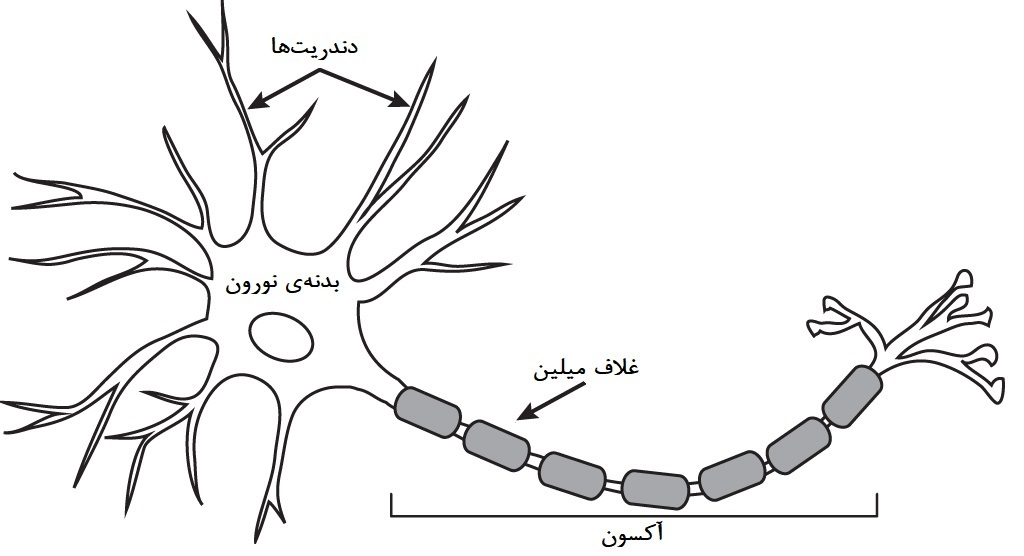
\includegraphics[width=0.7\linewidth]{neuron.jpg}
		\caption[NS]{
			اجزای تشکیل دهنده‌ی نورون\footnotemark.
		}
		\label{fig:neuron}
	\end{figure}
	
	% اینا همشون برعکس شدن (لاتین ها و اعداد. نسخه‌ی ۴ هست ولی برای درست نشون داده شدن برعکس نوشته شده)
	\RTLfootnotetext{
		خلق شده توسط
		Henley Casey 
		تحت مجوز
		BY-NC-SA CC
		نسخه ۰.۴.
	}
	
	
	نورون‌ها شامل یک لایه عایق هستند که موجب اختلاف پتانسیل مابین داخل و خارج نورون می‌شود. همچنین مجموعه‌ای از کانال‌های یونی\LTRfootnote{Ion Channels} نیز وجود دارند که نورون از طریق آنها با محیط بیرون یون‌هایی را تبادل می‌کند که این تبادلات موجب تغیر در میزان اختلاف پتانسیل نورون می‌شود. زمانی که اختلاف پتانسیل یک نورون از یک آستانه فراتر رود مجموعه‌ای از این کانال‌ها باز شده و موجب افزایش بسیار سریع اختلاف پتانسیل و سپس کاهش مجدد آن به میزان طبیعی می‌شود که به این پدیده، شلیک یا \gls{spike}\LTRfootnote{Spike} می‌گوییم. در زمان رخ دادن پدیده‌ی \gls{spike}، همراه با افزایش ناگهانی اختلاف پتانسیل در نورون، این اختلاف پتانسیل از طریق آکسون‌ها منتقل می‌شود و در سیناپس‌ها موجب آزاد شدن \gls{neurotransmitters}\LTRfootnote{Neurotransmitter} می‌شود که نتیجتا باعث افزایش اختلاف پتانسیل در دندریت‌های مجاور این سیناپس‌ها می‌شود. در این پروسه به نورونی که منشا اختلاف پتانسیل انتقال داده شده بوده است را \gls{pre}‌\LTRfootnote{Pre-synaptic Neuron} و نورونی را که این اختلاف پتانسیل به آن منتقل شده است، \gls{post}‌\LTRfootnote{Post-synaptic Neuron} مینامیم.
	
	نورون‌ها از نظر عملکرد به دو دسته‌ی کلی تقسیم می‌شوند؛ دسته‌ی اول نورون‌های تحریکی\LTRfootnote{Excitatory} هستند که در سیناپس‌هایشان انتقال‌دهنده‌های عصبی تحریکی مثل گلوتامیت\LTRfootnote{Glutamate} آزاد می‌شود و باعث بیشتر شدن اختلاف پتانسیل در \gls{post} می‌شود. دسته‌ی دوم نورون‌های مهاری هستند که در سیناپس‌هایشان انتقال دهنده‌های عصبی مهاری مثل گابا\LTRfootnote{GABA} آزاد می‌شود و باعث کمتر شدن اختلاف پتانسیل در \gls{post} می‌شوند
	\cite{Purves2001-ns}.
	
	
	\subsection{انعطاف پذیری نورونی}
	
	\gls{Neuroplasticity}\LTRfootnote{Neuroplasticity} را می‌توان به عنوان توانایی سیستم عصبی برای تغیر فعالیت خودش در پاسخ به محرک درونی یا خارجی با اعمال تغیراتی در ساختار، عملکرد و اتصالات خودش قلمداد کرد
	\cite{MateosAparicio2019}.
	همچنین می‌توان پدیده‌ی یادگیری را در موجودات زنده محصول وجود انعطاف پذیری نورونی در آنها دانست.
	
	از جمله تاثیراتی که در نتیجه‌ی انعطاف پذیری نورونی ایجاد می‌شود، می‌توان به تغیر میزان تاثیر تحریکی یا مهاری \gls{pre} روی \gls{post} اشاره کرد که در نتیجه‌ی تغیر در ساختار دندیت‌ها و آکسون‌ها رخ می‌دهد.
	از جمله مهم‌ترین ‌قوانین یادگیری در این مورد، \gls{hebb}‌\LTRfootnote{H‌ebbian Learning Rule} است که به واسطه‌ی فعالیت‌های دنالد هب\LTRfootnote{Donald Hebb} معرفی شده است.
	صورت \gls{hebb} به این صورت بیان شده است: «زمانی که آکسون نورون الف به اندازه‌ای به (دندریت) نورون ب نزدیک  بود که مکررا یا دائما باعث تحریک آن شود، برخی فر‌آیند‌ها و تغیرات متابولیکی در یکی یا هر‌دوی نورو‌ن‌ها باعث تغیراتی می‌شوند تا تاثیر نورون الف در تحریک شدن نورون ب افزایش یابد»
	\cite{hebb1949organization}.
	همچنین کارلا شاتز\LTRfootnote{Carla Shatz} اینگونه قانون هب را تفسیر می‌کند: «آنهایی که همزمان ضربه میزنند، به‌هم متصل‌هم می‌شوند»
	\cite{shatz1992developing}.
	هرچند‌ این تفسیر ممکن است باعث برداشت غلط شود؛ چراکه اگر دو نورون به معنی واقعی کلمه در یک لحظه شلیک کنند امکان اینکه شلیک یکی از آن نورون‌ها معلول شلیک نورون دیگر باشد وجود نخواد داشت. بیشتر از موضوع همزمانی، موضوع ارتباط علت و معلولی بین شلیک نورون‌ها است که دارای اهمیت است
	\cite{granger1969investigating}.
	
	
	در دهه ۱۹۹۰ میلادی، آزمایش‌هایی باعث مشخص شدن پایه‌های نوروفیزیولوژی قانون هب بر اساس \gls{stdp}\LTRfootnote{Spike-timing dependent plasticity (STDP)} شدند.
	\cite{caporale2008spike} 
	مشخص شد وقتی یک \gls{exc}، به یک نورون تجریکی دیگر متصل شده است، اگر \gls{pre} با فاصله‌ی زمانی ۴۰ میلی ثانیه یا کمتر نسبت به \gls{post} ضربه بزند، سیناپس‌های اتصال آن‌ها تقویت می‌شوند و اگر \gls{post} زودتر از \gls{pre} ضربه بزند، سیناپس‌های مرتبط با اتصال آن‌ها تضعیف خواهند شد. (شکل \ref{fig:stdp})
	بر اساس روابط کشف شده در تضعیف و تقویت سیناپس‌ها، می‌توان تغیرات میزان اثرگذاری نورون‌ها روی یکدیگر را به صورت زیر مدل‌سازی کرد به صورتی که $w$ میزان اثرگذاری یک نورون روی نورون دیگر، $\tau_\pm$ ثابت‌های زمانی  و $A_\pm$ میزان تغیرات وزنهای سیناپسی هستند
	\cite{gerstner2014neuronal}:
	\begin{align}
		\Delta w =
		\begin{cases}
			A_+(w).\exp(\frac{-|\Delta t|}{\tau_+})  & \text{\lr{if}}\; t_{pre} \leq t_{post}, \\
			A_-(w).\exp(\frac{-|\Delta t|}{\tau_-})  & \text{\lr{if}}\; t_{pre} > t_{post}.
		\end{cases}
		\label{eq:stdp}
	\end{align}
	
	
	\begin{figure}[H]
		\centering
		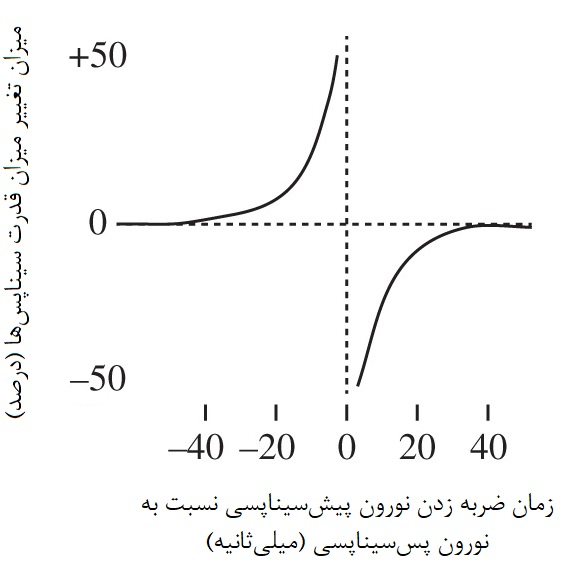
\includegraphics[width=0.7\linewidth]{stdp.jpg}
		\caption[NS]{
			میزان تقویت سیناپس ها در \gls{stdp} در فواصل زمانی مختلف برای اتصالات بین نورون‌های تحریکی.
		}
		\label{fig:stdp}
	\end{figure}

	همچنین پس از آن مشخص شده که این الگوی تغیرات برای سیناپس های مهاری متفاوت است و تغیرات وزن در هنگامی که فاصله‌ی زمانی بین ضربه زدن \gls{pre} و \gls{post} از حدود ۵ میلیٍ‌ثانیه کمتر باشد، بسیار ناچیز خواهد بود \cite{Haas2006}. (شکل \ref{fig:stdp-inh})
	
	\begin{figure}[H]
		\centering
		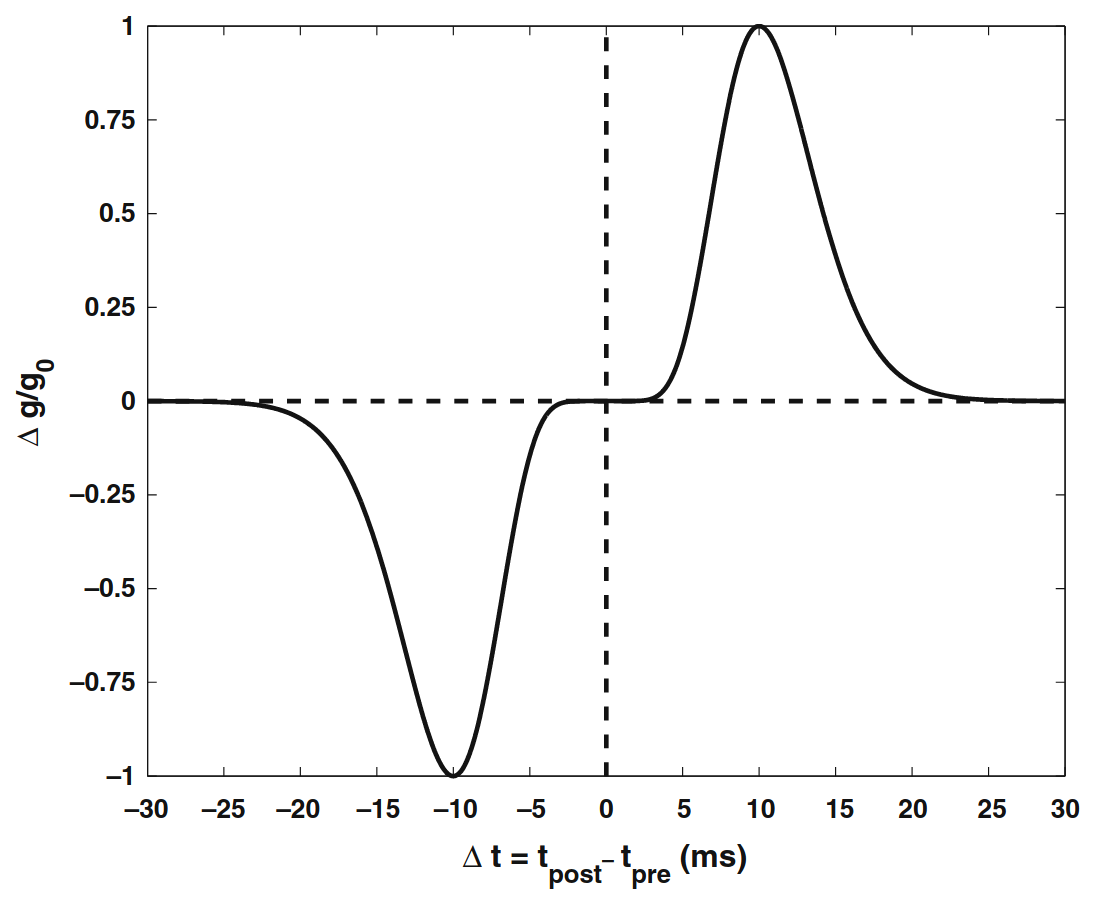
\includegraphics[width=0.7\linewidth]{stdp-inh.png}
		\caption[NS]{
			میزان تقویت سیناپس ها در \gls{stdp} در فواصل زمانی مختلف برای \gls{synapse}‌های مهاری.
		}
		\label{fig:stdp-inh}
	\end{figure}
	
	\subsection{سازوکار پاداش در مغز}
	\label{section:reward-in-brain}
	
	بخش بزرگی از یادگیری انسان در تعامل با محیط اتفاق می‌افتد. هر برون‌داد انسان تاثیری روی محیط پیرامونش گذاشته و محیط تغیر یافته، پس از آن تغیر، خود به عنوان یک درون‌داد از طریق سیستم عصبی محیطی درک می‌شود
	\cite{sutton1998reinforcement}.
	به توجه به درک انسان از محیط، پاداش یا تنبیه نیز برای آن در نظرگرفته می‌شود که این ساز‌و‌کار در مغز انسان بر عهده‌ی پیامرسان‌های عصبی\LTRfootnote{Neurotransmitter}  مثل \gls{dopamine}\LTRfootnote{Dopamine} است. 
	
	\begin{figure}[H]
		\centering
		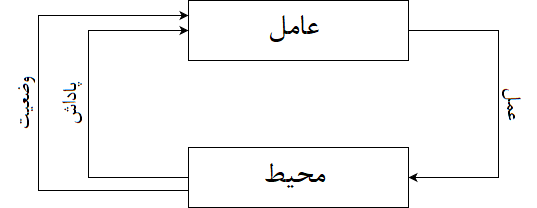
\includegraphics[width=0.7\linewidth]{rl.png}
		\caption[NS]{
			آثار \gls{agent} و محیط نسبت به یکدیگر
		}
		\label{fig:rl}
	\end{figure}
	
	تاثیر پاداش روی فعالیت اعصاب به این صورت است که برخی از نورون‌ها به این دسته از پیامرسان‌‌های عصبی حساس هستند و میزان غلظت آن‌ها روی فعالیت این دسته از نورون‌ها تاثیر گذار هستند و این تاثیر به گونه‌ای است که در صورتی که سیگنال پاداش دریافت شود، تغیرات وزن‌های اتصالات نورونی مشابه \gls{stdp} تغیر خواهند کرد؛ هرچند که میزان پاداش در شدت این تغیرات موثر است. همچنین در صورتی که سیگنال تنبیه دریافت شود تغیرات وزن‌های اتصالات بین نورونی برعکس \gls{stdp} تغیر خواهند کرد و میزان این تغیرات مشابه زمان پاداش وابسته به میزان شدت تنبیه خواهد بود.
	
	برای مدل‌سازی اثر سازوکار پاداش روی یادگیری می‌توان از روابط زیر استفاده کرد که در آنها $d$ میزان پاداش، $\delta$ تابع دیراک و $\tau_c$ به عنوان ثابت زمانی در نظر گرفته شده اند:
	
	\begin{align}
		\frac{dc}{dt} &= -\frac{c}{\tau_c} + STDP(\tau) \delta(t-t_{pre/post}) \\
		\frac{ds}{dt} &= cd
		\label{eq:rstdp}
	\end{align}
	
	
	\subsection{\gls{neocortex} و \gls{cc}}
	\gls{neocortex} یک قشر مغزی شش لایه در پستانداران است که وظیفه‌ی عملکرد‌های سطح بالایی همچون شناخت، حرکت، بینایی و زبان را برعهده دارد
	\cite{Lui2011}. نامگذاری لایه‌های \gls{neocortex} به ترتیب از بیرونی ترین لایه شماره ۱ تا درونی ترین لایه، لایه شماره ۶ می‌باشد.
	همچنین \gls{neocortex} شامل نورون های تحریکی و مهاری با نسبت تقریبی ۸۰ به ۲۰ می‌باشد
	\cite{noback2005human}.
	
	ساختار \gls{neocortex} علاوه‌بر اینکه شامل ۶ لایه افقی می‌باشد، شامل مجموعه ای از سازه‌های عمودی به نام \gls{cc} است که سطح مقطع بسیار کوچکی در ابعاد نیم میلی‌متر دارند و \gls{neocortex} از کنار‌هم قرار گرفتن این ستون‌ها شکل می‌گیرد
	\cite{Horton2005}.
	به صورت کلی، این ستون‌های کورتکسی از نظر ارتباط بین لایه‌ها الگوی‌های مشابه و تکرار شونده‌ای دارند که در تمام بخش های \gls{neocortex} مشابه یکدیگر هستند. \gls{ccc}\LTRfootnote{Canonical Cortical Circuit}، که توسط داگلاس و مارتین 
	\cite{Douglas2004}
	بیان شده، ارتباط بین بخش‌های مختلف را داخل و مابین ستون‌های کورتکسی نشان می‌دهد.
	(شکل \ref{fig:cc-doganmart})
	
	\begin{figure}[H]
		\centering
		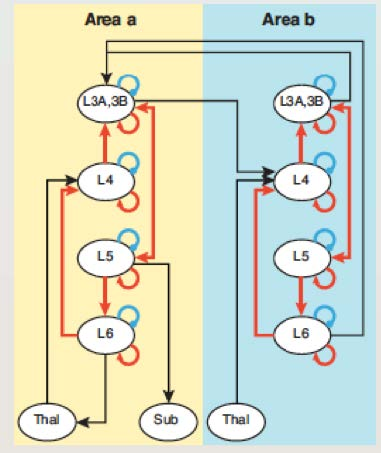
\includegraphics[width=0.5\linewidth]{cc-con.jpg}
		\caption[NS]{
			مدار کورتکسی استاندارد که توسط داگلاس و مارتین بیان شده است
			\cite{Douglas2004}.
			در این شکل پیکان‌های قرمز نشان دهنده‌ی اتصالات تحریکی و پیکان‌های آبی نشان دهنده‌ی اتصالات مهاری هستند. همانطور که در شکل نیز مشخص شده بیشتر اتصالات مهاری بین نورون‌های یک لایه‌ی مشخص هستند. همچنین پیکان‌های مشخص شده با رنگ مشکی نشانگر اتصالات بین دو ستون کورتکسی مجزا هستند.
		}
		\label{fig:cc-doganmart}
	\end{figure}
	
	
	\subsection{نورون‌های هرمی}
	
	\gls{pyramidal}\LTRfootnote{Pyramidal Neurons} نوعی\gls{multipolar}\LTRfootnote{Multipolar Neuron} هستند که در نواحی بسیاری از مغز حضور دارند و بخش اعظم نورون‌های تحریکی در نئوکورتکس را تشکیل می‌دهند \cite{Hawkins2016}.
	از جمله مهم‌ترین ویژگی‌های نورون‌های هرمی حضور دو گروه از دندریت‌ها به نام‌های \gls{apicalden}\LTRfootnote{Apical} و \gls{basalden}\LTRfootnote{Basal} در آن‌ها است.
	دندریت‌های رأسی معمولا اتصالاتی از راه دور هستند که تا بخش‌های دیگر مغز نیز می‌توانند پراکنده شده باشند و معمولا در سطح خارجی نئوکورتکس مستقر هستند \cite{MEGIAS2001527}. دندریت‌‌های پایه معمولا نزدیک به \gls{soma} هستند و فواصل زیادی را طی نمی‌کنند.
	
	\begin{figure}[H]
		\centering
		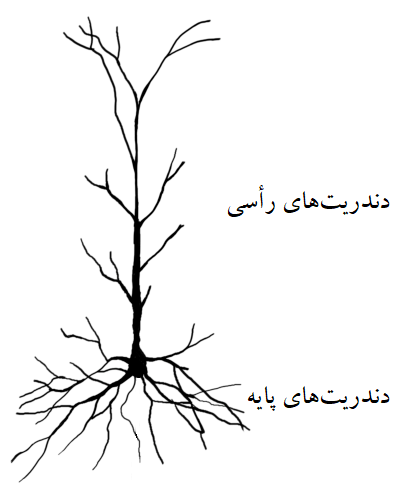
\includegraphics[width=0.5\linewidth]{pyramidal.png}
		\caption[NS]{
			نمایی از ساختار نورون‌های هرمی و مشخص شدن دندریت‌های رأسی و پایه در آن.
		}
		\label{fig:pyramidal}
	\end{figure}
	
	\section{مسئله‌ی \gls{binding}}
	
	در حوزه‌های علوم اعصاب، علوم شناختی و فلسفه ذهن مسئله‌ای تحت عنوان مسئله‌ی \gls{binding}
	\LTRfootnote{Binding Problem}
	یا \gls{combprob}
	\LTRfootnote{Combination Problem}
	مطرح می‌شود که در ادامه به پاره‌ای از موضوعات حول آن خواهیم پرداخت.
	
	\subsection{صورت مسئله‌ی \gls{binding}}
	
	مسئله‌ی \gls{binding} به چگونگی پردازش مفاهیم مجزا همچون اشیاء و ویژگی‌های انتزاعی و احساسی به صورت یک مفهوم گسترده‌تر تجمیع شده می‌پردازد
	\cite{REVONSUO1999123}.
	
	به صورت عمومی این مسئله به چگونگی در‌هم آمیختن مفاهیم مختلف درک شده و تجمیع آن‌ها به صورت یک تجربه‌ی واحد می‌پردازد
	\cite{Feldman2012}.
	همچنین دلیل اینکه از \gls{binding} به عنوان یک مسئله یاد می‌شود این است که هنوز به صورت کامل از سازوکار آن اطلاعی در دست نیست.
	
	\begin{figure}[H]
		\centering
		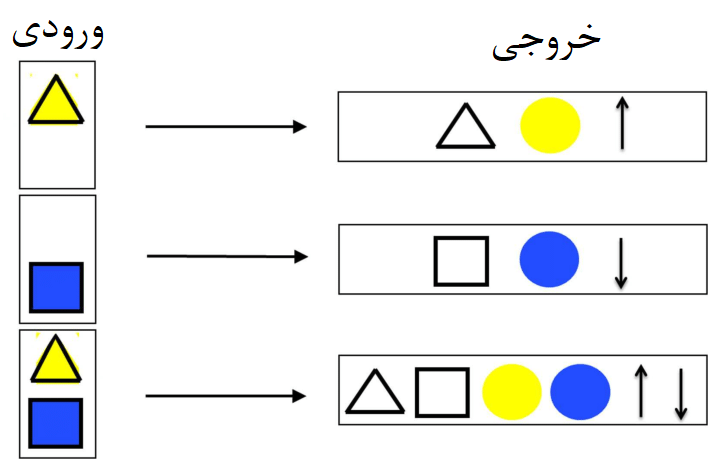
\includegraphics[width=0.7\linewidth]{binding.png}
		\caption[NS]{
			یک نمایش از تعریف کلاسیک \gls{binding} و چگونگی ادراک مفاهیم جامع توسط درک مفاهیم جزئی‌تر.
			\cite{velic2012}.
		}
		\label{fig:binding}
	\end{figure}
	
	
	\subsection{شواهد رخ‌دادن \gls{binding} در انسان}
	\label{subsection:binding-in-human}
	
	
	آنه تریسمن\LTRfootnote{Anne Treisman}
	و هیلاری اشمیت\LTRfootnote{Hilary Schmidt}
	آزمایشی را انجام دادند که در آن به مطالعه اثری با نام ترکیب‌های توهمی\LTRfootnote{Illusory Conjunctions}
	پرداختند که در آن آزمایش ویژگی‌های یک شئ به شئ دیگری منتسب می‌شود
	\cite{TREISMAN1982107}.
	بر اساس نظر تریسمن، علت این انتصاب اشتباه در ویژگی‌های اشیاء، حضور جدا از هم صفات در مراحل اولیه ادراکی است
	\cite{goldstein_2019}.
	اهمیت این موضوع از این جهت است که حالت ممکن دیگر آن است که یک شئ نه به صورت صفات جداگانه، بلکه به صورت یک ماهیت کامل حاضر شود. این در حالی است که رخ دادن مسئله‌ی \gls{binding} در مغز مستلزم حضور ویژگی‌ها و صفات به صورت جدا از هم می‌باشد که این آزمایش نشانگر اتفاق افتادن \gls{binding} در مغز است. همچنین گروهی دیگر برای نشان دادن مصادیق انقیاد در انسان به نمونه‌های شناختی آن همچون \gls{Bind} کردن دانش معنایی\LTRfootnote{Semantic Knowledge} به شهود، مقید کردن متغیر‌ها در زبان و استنتاج اشاره می‌کنند \cite{greff2020binding}.
	
	
	\section{\gls{snn}}
	\gls{ann}\LTRfootnote{Artificial Neural Networks} بر پایه دینامیک‌های بسیار ساده شده مغز ساخته شده‌اند و به عنوان یک ابزار محاسباتی قوی برای حل بسیاری از مسائل استفاده می‌شوند
	\cite{TGNN}. 
	\gls{snn}\LTRfootnote{Spiking Neural Networks} نوعی از شبکه‌های عصبی مصنوعی هستند که در آن ارتباط بین نورون‌ها توسط ضربه‌ها و سیناپس‌ها  با وزن‌های متغیر، مطابق با مشاهدات زیستی تعریف شده‌اند
	\cite{ghosh2009spiking}. 
	از جمله مهمترین ویژگی هایی که در \gls{snn} در نظر گرفته شده، بعد زمان است
	\cite{Mozafari2019}
	که این مورد در شبکه‌های عصبی کلاسیک در نظر گرفته نمی‌شده. در \gls{snn} اطلاعات می‌توانند در زمان‌های مختلفی منتقل شوند و زمان خود در مفهوم منتقل شده نقش مهمی را بازی می‌کند
	\cite{SNN1997}.
	
	برای شبیه‌سازی این گونه از شبکه‌های عصبی، سازوکار نورون‌های زیستی به روش‌‌های گوناگونی مدل‌سازی شده‌اند که ازجمله ساده ترین‌ها که در عین‌حال کارایی بسیار مناسبی را دارد مدل نورونی \gls{lif}\LTRfootnote{Leaky integrate-and-fire} است که در ادامه به آن خواهیم پرداخت.
	
	
	\subsection{مدل نورونی \gls{lif}}
	در مدل نورونی \gls{lif} تلاش شده تا ویژگی‌ها و خواص مهم نورون‌های بیولوژیکی لحاظ شوند. در این نورون‌ها با وارد شدن ضربه‌های تولید شده توسط نورون‌های پیش‌سیناپسی به نورون، اختلاف پتانسیل آن افزایش می‌یابد (تجمیع) و در صورت رسیدن اختلاف پتانسیل به یک آستانه‌ی مشخص، این نورون خود ضربه‌ای تولید می‌کند (آتش) که توسط اتصالات بین نورونی به نورون‌های پس‌سیناپسی منتقل می‌شوند. همچنین در گذر زمان اختلاف پتانسیل نورون به مرور در حال کاهش به سمت یک میزان مشخص اختلاف پتانسیل است (نشتی) که به آن اختلاف پتانسیل استراحت می‌گوییم
	\cite{gerstner2014neuronal}.
	
	ساز‌وکار بیان شده برای تغیرات اختلاف پتانسیل را در این مدل نورونی می‌توان به صورت معادلات دیفرانسیل بیان شده در رابطه‌ی \ref{eq:lif} بیان کرد که در آن $u$ اخلاف پتانسیل فعلی نورون، $u_{rest}$ اختلاف \gls{rest}، $I(t)$ جریان ورودی به نورون و $R$ مقاومت الکتریکی قشای نورون را نشان می‌دهند
	\cite{gerstner2014neuronal}.
	
	\begin{align}
		\tau . \frac{du}{dt} = -(u - u_{rest}) + R . I(t) 
		\label{eq:lif}
	\end{align}

	\subsection{\gls{rl} در شبکه‌های عصبی ضربه‌ای}
	
	پیش‌تر در بخش \ref{section:reward-in-brain} به سازوکار پاداش در مغز انسان پرداختیم و مدل آنرا نیز بررسی کردیم. از سازوکار مطرح شده در \gls{snn} برای یادگیری تقویتی استفاده می‌شود تا مدل با توجه به الگوی فعالیتش در طول زمان و در مجاورت محیط، که منجر به دریافت پاداش و تنبیه می‌شود، آموزش داده شود و به رفتار آن به سمتی متمایل شود که بیشترین پاداش را در طول زمان دریافت کند. قانون یادگیری حاصل از استفاده از این مدل را \gls{rstdp}\LTRfootnote{Reward-modulated spike-timing dependent plasticity} می‌نامند.
	
	برای به کار گرفتن یادگیری تقویتی در یک مدل، باید بر اساس شرایط محیط فرضی شبیه‌سازی شده و رفتار عامل در آن، یک مقدار برای میزان پاداش یا تنبیه محاسبه شود تا بتوان به عنوان مقدار دوپامین در مدل از آن استفاده کرد.
 	
	
	\chapter{طرح مسئله}
	
	در این فصل پس از یک مرور مختصر درباره‌ی مسئله‌ی \gls{binding} به اهمیت مدل‌سازی مسئله‌ی \gls{binding} و مسائلی که درک بیشتر ما از این موضوع آن‌ها را نیز تحت تاثیر قرار خواهد داد، خواهیم پرداخت که از‌جمله آن‌ها می‌توان به هوش مصنوعی و درک بهتر ساز‌وکار مغز اشاره کرد.
	
	\section{مسئله‌ی \gls{binding}}
	
	به صورت کلی مسئله‌ی انقیاد به ظرفیت ما برای یک‌پارچه کردن اطلاعات در طول زمان، فضا ، ویژگی‌های مختلف و ایده‌ها است. مسئله‌ی انقیاد به صورت سه مسئله‌ی مجزا قابل بررسی است و در هریک از تحقیقات مختلف مسئله‌ی مورد بررسی به یکی از این سه دسته متعلق است \cite{Treisman1999}:
	
	\begin{itemize}
		\item چگونگی تشخیص مفاهیم مقید شده به عنوان یک مفهوم واحد  و تفکیک آن‌ها از مفاهیمی که مقید به مفاهیمی دیگر هستند.
		\item چگونگی کد‌گذاری انقیاد در مغز و این‌که چگونه در مغز به آن رجوع می‌شود.
		\item چگونگی تشخیص ارتباط صحیح بین مفاهیم  مقید شده و یک شی بخصوص.
	\end{itemize}

	بسیاری از پژوهش‌های در موضوع مسئله‌ی انقیاد در موضوع دوم هستند. در پژوهش حاضر مفهوم مورد بررسی چگونگی رخ دادن انقیاد در مغز و در مقیاس ارتباطات نورونی است که در دسته‌ی دوم، یعنی چگونگی کدگذاری  در مغز مرتبط می‌شود \cite{Treisman1999}. درواقع مسئله‌ی اصلی چگونگی یکپارچه شدن مفاهیم مجزا ولی مرتبط در قالب یک مفهوم واحد در ساختار نورون‌ها و اتصالات بین آن‌ها است.
	
	
	
	\section{مشکلات موجود حاضر}
	در زمینه‌ی شبکه‌های عصبی، مسئله‌ی انقیاد تنها یک مسئله‌ی حل نشده درباره‌ی ادراک نیست؛ بلکه تشخیص محدودیت‌های حال حاضر شبکه‌های عصبی مصنوعی موجود نیز بخشی از مسائلی است که محققان را مشغول خود کرده است.
	با توجه به چالش‌های حال حاضر، درک چگونگی اتفاق افتادن \gls{binding} در مغز، از اهمیت بالایی برخوردار است؛ زیرا با توجه به اهمیت و میزان تاثیر \gls{binding} در آگاهی و درک موجود زنده از محیط خود، به این موضوع در مسائلی همچون درک و شبیه‌سازی هوش انسانی که یکی از چالش‌های هوش مصنوعی است، نیاز است.
	
	در راستای دست‌یابی به سیستم‌های هوشمند فعالیت‌های بسیاری انجام شده است که از جمله‌ موفق ترین و موثر ترین روش‌های حاضر، استفاده از شبکه‌های عصبی مصنوعی است که یک روش الهام گرفته شده از \gls{nervousSystem} انسان است و در حال حاضر به صورت گسترده مورد استفاده قرار گرفته‌اند. این روش در  عین این‌که در شرایط مناسب از بهره‌وری بسیار خوبی برخوردار است و امکان دست‌یابی به نتایج بسیار خوبی را در مدل‌سازی آماری داده‌های جهان دارد، به میزان داده‌ی بسیار زیادی برای آموزش نیاز دارد، در انتقال مفاهیم از پیش آموخته شده به مسائل جدید نیز با مشکل مواجه است و امکان تعمیم و عمومی سازی مسائل آموخته‌شده را ندارند.
	از جمله اصلی ترین دلایل مشکلات و محدودیت‌های موجود در شبکه‌های عصبی مصنوعی، ناتوانی آن‌ها در شکل‌دهی، بازنمایی و ارتباط بین مفاهیم و موجودیت‌ها است. به خوبی نشان داده شده است که درک انسان حول اشیاء شکل گرفته است که این اشیاء می‌توانند به صورت مستقل پردازش شوند و به حالت‌های بسیار زیادی دوباره با یکدیگر ترکیب شوند و این مسئله به انسان امکان تعمیم درک خود به مسائل فراتر از تجربیاتش را می‌دهد که این ساز‌وکار همان رویه مورد بررسی در مسئله‌ی \gls{binding} است
	\cite{greff2020binding}.
	
	ارتباطات بین مفاهیم در رخ دادن انقیاد به شکل‌های مختلفی ممکن است؛ همچون رابطه‌ی علّی، ارتباط سلسه‌مراتبی و ارتباط مقایسه‌ای. تعریف مفاهیم در قالب انواع مختلف این روابط می‌تواند تاثیراتی روی مفاهیم‌شکل گرفته داشته باشد. همچنین مورد مهم‌این است که این روابط به صورت مجزا از هم و مستقل مفاهیم شکل گرفته‌ از اشیا باشند. انواع مختلف ارتباطات قابل پیاده‌سازی نیز، خود یکی از چالش‌های موجود در حل این مسئله است.
	
	\section{عملکرد شبکه‌های عصبی ضربه‌ای در مسائل مطرح شده}
	شبکه‌های عصبی ضربه‌ای در مقایسه با شبکه‌های عصبی کلاسیک از توجیه زیستی بسیار بیشتری برخوردار هستند و در آن‌ها جزعیات نورون‌های زیستی بسیار بیشتر در نظر گرفته شده است که این موضوع پتانسیل‌های این دسته از شبکه‌هارا نیز تحت تاثیر قرار می‌دهد. در این دسته از شبکه‌ها به دلیل انتقال داده‌ها با در نظر گرفتن زمان و در قالب ضربه (بجای عدد در شبکه‌‌های عصبی کلاسیک) امکان درک مفاهیم به صورت اشیاء بجای مدل‌سازی آماری در آن‌ها بسیار محتمل‌تر است و به همین دلیل این امکان وجود دارد که بتوان در این دسته از شبکه‌های عصبی سازوکاری را تحت شرایط مشخصی به‌وجود آورد که در آن مسائل و مشکلات مطرح شده دیگر رخ ندهند و به عبارتی در این دسته از شبکه‌های عصبی می‌توان انتظار اتفاق افتادن \gls{binding} را داشت.
	
	\section{تعریف مسئله}
	همواره شبیه‌سازی و درک ساختار‌های موجود در مغز انسان جزو مسائل مورد اهمیت برای انسان‌ها بوده است و در دهه‌های اخیر نیز با رشد و گسترش قدرت محاسباتی و علومی چون هوش مصنوعی و علوم اعصاب این اهداف بسیار در دسترس تر از پیش به نظر میرسند و فعالیت‌های بسیاری نیز در دهه های اخیر در رابطه با این موضوع آغاز شده است که از جمله‌ی آن‌ها می‌توان به پروژه مغز آبی\LTRfootnote{Blue Brain Project} و پروژه‌ی مغز انسان\LTRfootnote{Human Brain Project (HBP)} اشاره کرد.
	
	چنانچه پیشتر مطرح شد، مسئله‌ی \gls{binding} به عنوان یکی از مهمترین مسائل در شناخت مغز و هوش مصنوعی، که تقریبا در تمام فعالیت‌های شناختی پستانداران در حال رخ دادن است، برای شبیه‌سازی در شبکه‌های عصبی مصنوعی کلاسیک که صرفا نرخ ضربه با کد می‌کنند\LTRfootnote{Rate-coding} با محدودیت‌هایی مواجه است \cite{vonderMalsburg1999} که این موضوع را در دسته‌ی مسائل حل نشده قرار داده است. ولی در سال‌های اخیر با افزایش قدرت پردازشی و پیشرفت شبکه‌های عصبی ضربه‌ای‌، امید است تا بتوان با استفاده از این نسل از شبکه‌های عصبی مصنوعی مسیر جدیدی در درک و شبیه‌سازی مسئله‌ی \gls{binding} را در پیش گرفت که به نتایج بهتری نسبت به انواع کلاسیک در آن رسید.
	
	همچنین استفاده شبکه‌های عصبی ضربه‌ای این امکان را برای ما فراهم می‌کند که در ساختار و توپولوژی شبکه نیز از ساختار‌های طبیعی مغز بیش از پیش الگوبرداری کرد. این موضوع از این جهت  حائز اهمیت است که \gls{binding} در مغز پستانداران در حال رخ دادن است و هرچه بیشتر مکانیز ها و شبکه‌ی شبیه‌سازی شده، بیشتر شبیه نمونه‌ی طبیعی خود باشند احتمال رخ دادن \gls{binding} نیز در شبیه‌سازی بیشتر خواهد بود.
	
	در مطالعه‌ی پیش‌رو در تلاش خواهیم بود تا با استفاده از شبکه‌های عصبی ضربه‌ای و الگو برداری از ساختار و توپولوژی مغز پستانداران یک شبکه‌ی عصبی را شبیه‌سازی کنیم و در آن وجود آثاری از رخ دادن \gls{binding} را بررسی کنیم.
	
	
	\chapter{تحقیقات پیشین}
	
	در این فصل مجموعه‌ای از تحقیقات انجام شده پیرامون مسئله‌ی \gls{binding} و نظریه‌هایی پیرامون چگونگی رخ دادن آن در مغز و تلاش‌هایی برای مدل‌سازی آن به صورت محاسباتی را بررسی خواهیم کرد.
	
	\section{رخ دادن انقیاد در انسان}
	همانطور که در بخش \ref{subsection:binding-in-human} نیز اشاره شد، تحقیقی توسط آنه تریسمن و هیلاری اشمیت صورت گرفته که نشان می‌دهد ویژگی‌های مختلف یک شی در مغز به صورت مجزا از هم پردازش می‌شوند. \cite{TREISMAN1982107}
	
	آن‌ها صفحه‌ای را به شرکت‌کننده ارائه می‌کردند که در آن چهار شکل با رنگ‌های مختلف به همراه دو عدد مشکی وجود داشت. آن‌ها این صفحه را به مدت ۰.۲ ثانیه نشان می‌دادند و پس از آن یک صفحه با نقاط مشکی تصادفی نمایش داده می‌شد. هدف از نمایش صفحه با نقاط مشکی، از بین بردن هر نوع رد ادراکی از محرک پیشین بود. سپس از شرکت‌کنندگان خواسته می‌شد تا اعداد و اشکال نمایش داده شده را توصیف کنند.
	
	در حدود یک پنجم کوشش‌های شرکت کنندگان ترکیب شدن ویژگی‌های اشکال نمایش داده شده دیده می‌شد. برای مثال رنگ یا اندازه‌ی دو شکل با یکدیگر جابجا گزارش می‌شدند.
	
	بر اساس نظر تریسمن، علت شکل گیری این پدیده، جدا بودن صفات در مرحله‌ی پیش توجهی از یکدیگر و مقید نبودن آن‌ها به شی‌ بخصوصی است. \cite{goldstein_2019}
	
	\section{پیدایش \gls{binding} در گروه‌های چندزمانی}
	اگوچی و همکارانش در پژوهشی
	\cite{EGUCHI2018a}
	با ساخت یک شبکه‌ی عصبی سلسله مراتبی که لحاظ کردن تاخیر انتقال آکسونی\LTRfootnote{Axonal Transmission Delay} در آن باعث شده تا در زیرجمعیت‌های آن \gls{polychron}\LTRfootnote{Poly-chron Groups}\cite{Izhikevich2006-dy} شکل بگیرند که هریک از آن‌ها به یک الگوی تصادفی با توزیع \gls{poisson} حساس شده بودند، نشان دادند که \gls{binding} بین مفاهیم دیداری سطح پایین و سطح بالا به مرور زمان شکل می‌گیرد که در این شبکه هریک از این مفاهیم در قالب فعالیت یک گروه چندزمانی در نظر گرفته شده بودند.
	
	مثالی از نمود بسیار ساده‌ی \gls{binding} در این شبکه در شکل \ref{fig:eguchi-binding} نشان داده شده است که در آن به دلیل وجود تاخیر در انتقال، وقتی چند مفهوم که هریک به یک یا مجموعه‌ای از نورون‌ها مقید شده اند، در فواصل زمانی مشخصی به شبکه داده شوند باعث فعال شدن یک مفهوم سطح بالاتر که شامل مفاهیم سطح پایین‌تر نیز می‌باشد، می‌شوند. 
	
	\begin{figure}[H]
		\centering
		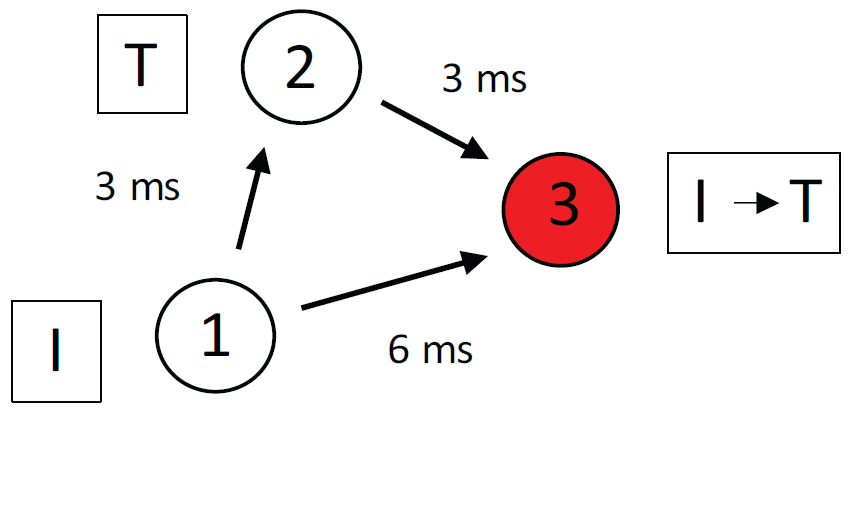
\includegraphics[width=0.7\linewidth]{poly-bind.png}
		\caption[NS]{
			یک مثال فرضی از انقیاد در سطح نورونی که در آن نورون شماره ۱، یک ویژگی سطح پایین مثل یک خط عمودی را نمایندگی می‌کند و نورون شماره ۲ نیز یک ویژگی سطح بالاتر مثل تصویر حرف T را نمایندگی می‌کند و نورون شماره ۳ انقیاد را مشخص می‌کند. به عبارتی نورون ۳ فعال می‌شود اگر و تنها اگر نورون ۱ در فعال شدن نورون ۲ نقش مستقیم داشته باشد.
		}
		\label{fig:eguchi-binding}
	\end{figure}
	
	پدیده‌ی مطرح شده می‌تواند بین گروه‌های چندزمانی نیز رخ دهد. به عبارتی \gls{binding} می‌تواند بین گروه‌های چندزمانی که نماینده‌ی یک مفهوم مستقل هستند رخ دهد و با یک گروه چند زمانی دیگر نمایندگی شود که نمونه‌ی آن نیز در شکل \ref{fig:eguchi-binding-group} قابل مشاهده است.
	
	\begin{figure}[H]
		\centering
		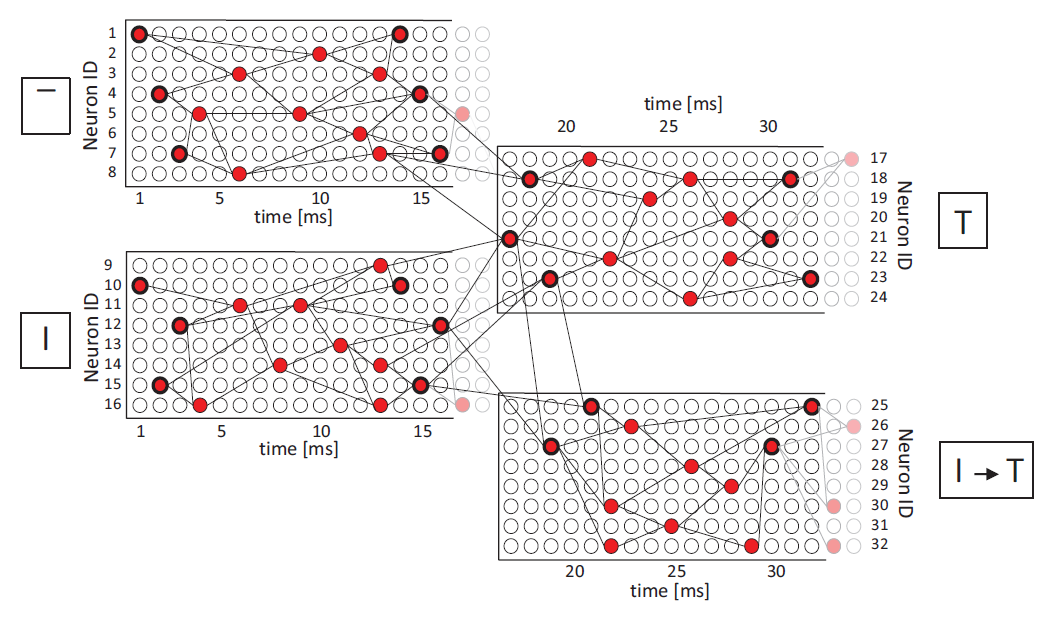
\includegraphics[width=0.7\linewidth]{poly-group-bind.png}
		\caption[NS]{
			نمود رخ دادن مثال ذکر شده در شکل \ref{fig:eguchi-binding}  از \gls{binding} در گروه های چند زمانی.
		}
		\label{fig:eguchi-binding-group}
	\end{figure}
	
	\section{ستون‌های کورتکسی، واحد‌های مستقل محاسباتی}
	هاوکینز در کتابی \cite{Hawkins2021-rq} که حاصل از مجموعه تحقیقات هاوکینز و همکارانش
	\cite{Hawkins2016, Hawkins2017, Lewis2019}
	بود، با فرض اینکه ستون‌های کورتکسی در سراسر نئوکورتکس ساختار‌های مشابهی دارند و عملکرد آن‌ها صرفا به دلیل تفاوت ورودی‌های آن‌ها است \cite{Mountcastle1978} یک مدل نورونی برای حل مسئله‌ی \gls{binding} پیشنهاد داد. با فرض اینکه هر ستون کورتکسی مسئولیت درک مفهومی را بر عهده دارد و با علم بر این که می‌تواند بین لایه‌های متناظر برخی ستون‌های کورتکسی با فاصله‌ی مکانی بالا، \gls{longdistancecon}\LTRfootnote{Long-distance connections} شکل بگیرد، این فرضیه را مطرح کرد که این اتصالات از راه دور می‌توانند به وجود آورنده‌ی نوعی مکانیزم رای‌گیری باشند که نهایتا موجب شکل گیری \gls{binding} در مغز می‌شوند.
	
	برای انجام شدن رای گیری، هر ستون کورتکسی با توجه به داده‌های ورودی خود، در صورت حضور مجموعه‌ای از مفاهیم فعال خواهد بود و برای دیگر مفاهیم فعالیت کمتری خواهد داشت. با استفاده از اتصالات از راه دور هر ستون کورتکسی فعالیت و عدم فعالیت خود را به دیگر ستون‌های کورتکسی مخابره می‌کند و در ستون‌های کورتکسی دیگر، مفاهیم محتمل‌تر، مفاهیم با احتمال پایین‌تر را خنثی کرده و نهایتا از روی فعالیت چندین ستون کورتکسی یک مفهوم جامع‌تر حاصل شده از فعالیت دیگر ستون‌ها شکل می‌گیرد. پیش از این نیز تحقیقاتی این احتمال را مطرح کرده بودند که انشعابات مختلف دندریتی می‌توانند به عنوان تشخیص دهنده‌های الگو های مستقل از هم عمل کنند \cite{POIRAZI2003989, Polsky2004} که در این پژوهش نیز این مورد فرض شده که این الگو‌های مستقل درواقع بیانگر احتمالات مختلف هستند و با توجه به اینکه بیشتر جمعیت نورون‌هیا تحریکی را در نئوکورتکس، نورون‌های هرمی تشکیل می‌دهند، مخابره‌کردن این پیام‌های از راه دور درواقع بر عهده‌ی دندریت‌های رأسی و دندریت‌های پایه‌ با فاصله‌ی بیشتر است. به این صورت که افزایش اختلاف پتانسیل از طریق این دسته‌از دندریت‌ها باعث نزدیکتر شدن نورون به \gls{thresh}‌ی ضربه می‌شوند ولی باعث ضربه نمی‌شوند و صرفا شرایط را برای رسیدن به آستانه‌ی ضربه از طریق فعالیت دندریت‌های نزدیکتر به مبدا، فراهم می‌کنند.
	
	مدل پیشنهادی آن‌ها (شکل \ref{fig:hawkins2017}) برای ستون‌های کورتکسی، یک مدل دو لایه‌ است که ورودی ستون کورتکسی وارد یکی از لایه‌ها شده و از آن لایه پس از پردازش به لایه‌ی دیگر منتقل می‌شود و سپس از لایه‌‌ی دوم از طریق اتصالات از راه دور به لا‌‌یه‌های دوم دیگر ستون‌های کورتکسی منتقل می‌شوند. همچنین آن‌ها مجموعه‌ای از اتصالات بازخورد\LTRfootnote{F‌‌‌eedback Connections} را نیز از لایه‌ی دوم به لا‌یه‌ی اول تعریف کردند که وظیفه‌ی آن‌ها ارائه‌ی یک پیش‌نمایش از مفهوم‌ شکل گرفته در لايه‌ی دوم است که باعث تعادل و هماهنگی بین دو لایه‌ می‌شود. در مطالعه‌ی صورت گرفته توسط ایشان\cite{Hawkins2017} مفهوم مورد بررسی، درک موقعیت‌های مکانی از روی داده‌های مربوط به حس لامسه بوده است و انتظار آن‌ها شکل گرفتن یک فعالیت با ثبات متناظر با مکان مورد لمس، در لایه‌ی دوم بدون لحاظ شدن حالت خود شئ (زاویه و جهت) بوده. 
	
	\begin{figure}[H]
		\centering
		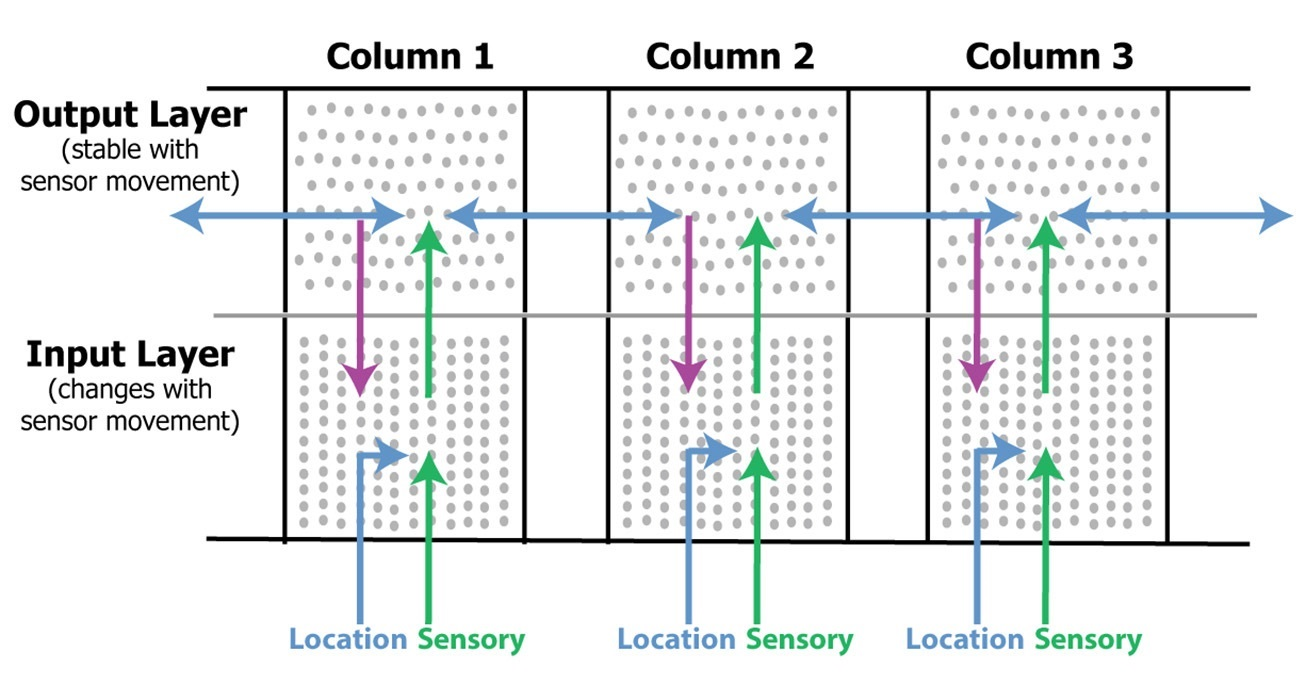
\includegraphics[width=1.0\linewidth]{hawkins2017.jpg}
		\caption[NS]{
			مدل پیشنهادی در مطالعه‌ی صورت گرفته \cite{Hawkins2017} برای درک موقعیت‌های مکانی با استفاده از داده‌های مربوط به لامسه و حرکت انگشت‌ها.
		}
		\label{fig:hawkins2017} 
	\end{figure}

در شبکه‌ی ارائه شده توسط آن‌ها برای شبیه‌سازی نورون‌ها از مدل نورونی  HTM (که به عبارت «\gls{htm}\LTRfootnote{Hierarchical Temporal Memory}» دلالت دارد) استفاده شده است \cite{HTM2011}. همانطور که از عنوان این مدل‌های نورونی مشخص است، HTM ها نورون‌هایی حافظه محور هستند. آن‌ها روی مجموعه‌ی بسیار بزرگی از داده‌های زمانی اموزش داده شده‌اند و مجموعه‌ی بزرگی از دنباله‌ها و الگوی‌های رفتاری را در خود ذخیره می‌کنند. حافظه‌ی این دسته از نورون‌ها دارای سازماندهی سلسله مراتبی است و ذاتاً مبتنی بر زمان است.

یکی دیگر از ویژگی‌های این مدل نورونی آن است که در ورودی‌های آن تفاوت بین دندریت‌های رأسی و پایه در نظر گرفته شده است و تلاش شده تا رفتار نورون‌های هرمی به صورت دقیق‌تر و نزدیکتر به حالت زیستی آن مدل‌سازی شوند. هرچند با وجود این‌که این مدل نسبت به شبکه‌های عصبی مصنوعی کلاسیک، شباهت بیشتری به نورون‌های زیستی دارد، ولی به اندازه‌ی شبکه‌های عصبی ضربه‌ای مشابه با نورون‌های زیستی نیستند.

\section{استفاده‌ از مدل مبتنی بر ستون کورتکسی در شبکه‌های عصبی}
در پژوهشی فردریک الکساندر\LTRfootnote{Frédéric Alexandre} و همکارانش یک واحد محاسباتی  بسیار ساده‌ی الهام گرفته شده از ستون‌های کورتکسی برای استفاده در شبکه‌های عصبی ارائه کردند \cite{Alexandre1991}. آن‌ها از این واحد در یک شبکه‌ی عصبی چند لایه برای \gls{patternrec} استفاده کردند.

آن‌ها برای این واحد محاسباتی، \gls{af}\LTRfootnote{Activation Function} و قانون یادگیری مختص به خود را ارائه دادند. آن‌ها برای مدل سازی یک ستون‌کورتکسی از \gls{tt} \LTRfootnote{Truth Table} استفاده کردند و حالت‌های مختلف خروجی ستون‌های کورتکسی را به نسبت ورودی‌های مختلف در آن لیست کردند و نهایتا یک تابع فعال‌ساز هماهنگ با آن داده‌ها را ارائه دادند. 

آن‌ها از این مدل برای تشخیص گفتار و تصویر استفاده کردند و در برخی از حالت‌ها این مدل عمل‌کرد بسیار مناسبی را از خود نشان داد ولی مدل آن‌ها به دلیل ساده سازی بسیار زیاد با رفتار نورون‌های زیستی فاصله‌ی بسیار زیادی دارد.


\section{استفاده از \gls{gnn} برای تشکیل انقیاد}
در پژوهشی صادقی و همکارانش با استفاده از یک معماری \gls{enc-dec}ی\LTRfootnote{Encoder-decoder} مولد\LTRfootnote{Generative} که نگاه خود را تطبیق می‌دهد و بین ویژگی‌ها با استفاده از استنتاج پس‌نگر انقیاد ایجاد می‌کند، الگو‌های حرکتی زیستی را مدل‌سازی کرده اند \cite{Sadeghi2021}.

آن‌ها در ابتدا مدلی را آموزش دادند که حرکت‌های زیستی پویا یا دیگر الگوی‌های حرکتی دارای هارمونی را یادبگیرد. سپس داده‌های ورودی را کمی درهم ریخته‌ کرده و خطای پیش‌بینی را بر روی یک ماتریس انقیاد، که یک لایه‌ی عصبی نمایانگر انقیاد ویژگی‌ها است، ذخیره می‌کنند. علاوه‌ بر این، آن‌ها خطا را به سمت نورون‌های نماینده‌ی دیدگاه مدل نشر می‌دهند که وظیفه‌ی این نورون‌ها ترجمه‌ی مقادیر ورودی به چارچوب‌های مرجع (یک دستگاه مختصاتی که در ان مکان، جهت و دیگر ویژگی‌های یک پدیده سنجیده می‌شود) است.

\begin{figure}[]
	\centering
	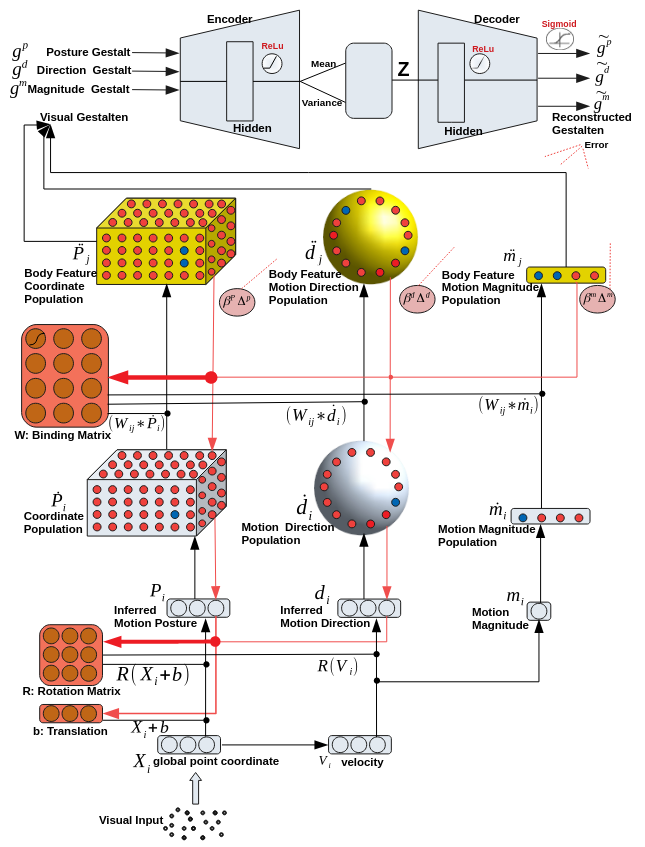
\includegraphics[width=0.8\linewidth]{gnn.png}
	\caption[NS]{
		مدل رمگذار-رمزگشای مولد ارائه شده در  \cite{Sadeghi2021}.
	}
	\label{fig:gnn}
\end{figure}

ارزیابی‌ها نشان دادند که این فرآیند استنتاج، انقیاد را برای الگو‌های شناخته‌شده‌ی حرکتی زیستی به وجود می‌آورند و یک درک گشتالتی\LTRfootnote{Gestalt}  تشکیل می‌دهند.
	
	همچنین آن‌ها این احتمال را مطرح کردند که ممکن است مدل ارائه شده توسط آن‌ها باید بتواند برای انقیاد بین مفاهیم \gls{gestalt}ی در دیگر حوزه ها نیز موثر باشد.
	
	
	\chapter{مدل پیشنهادی، آزمایش‌ها و نتایج}
	
	با توجه به مدل ارائه شده توسط هاوکینز و همکارانش و مشخص بودن اهمیت ستون‌های کورتکسی در شکل گیری شناخت و شکل گیری انقیاد، استفاده از این ساختار در طراحی آزمایشی به منظور مدل‌سازی و بررسی انقیاد در مغز می‌تواند تصمیم درستی باشد. همچنین با توجه به اینکه مدل مذکور یک مدل الهام گرفته شده از ساختار زیستی مغز است، و \gls{snn} نیز مشابه با آن، روشی الهام گرفته از ساختاز طبیعی مغز است، می‌تواند گزینه‌ی مناسبی برای مدل‌سازی نورون‌ها باشد. از این رو قصد داریم در ادامه‌ی این فصل مدلی مبتنی بر \gls{snn} با الهام از ساختار ستون‌های کورتکسی طراحی کنیم و شکل گیری انقیاد در آن را بررسی کنیم و در نهایت نیز نتایج حاصل از این تحقیق را بیان خواهیم کرد.
	
	\section{مدل پیشنهادی}
	
	مدل ارائه شده در این بخش شامل یک شبکه‌ی متشکل از سه ستون کورتکسی و ارتباطات مابین آنهاست. همچنین دو جمعیت با فعالیت از پیش مشخص شده نیز برای وارد کردن اطلاعات ورودی به شبکه مورد استفاده قرار می‌گیرند. فعالیت روی جمعیت‌های ورودی به دو وضعیت تقسیم شده است که در هریک نیمی از نورون‌ها نسبت به دیگر نورون‌ها فعالیت بیشتری دارند که بین این دو مجموعه از نورون‌های فعال به ازای هر وضعیت هیچ اشتراکی وجود ندارد که به عبارتی هر جمعیت از ورودی‌ها در هر زمان یک الگوی فعالیت از دو الگوی فعالیت ممکل را دارند. دو جمعیت ورودی همواره از نظر الگوی فعالیت مشابه یکدیگر هستند و زمان تغیر الگوی فعالیت نیز همزمان با یکدیگر الگو‌های فعالیتشان تغیر می‌کنند. این دو جمعیت ورودی نمایانگر دو ورودی سنسوری هستند هستند که با تغیر محیط عامل، الگوی فعالیت آن‌ها نیز تغیر می‌کند. برای مثال اگر فرض کنیم عامل در محیطی قرار دارد که دو ورودی سنسوری (مثل شنیدار و لامسه) به دلیل حضور عامل توسط عامل دریافت می‌شود، هز جمعیت متناظر با یکی از ورودی‌ها خواهد بود که هردو همزمان یا الگوی متناظر با حس کردن موجودیت اول را نشان‌ می‌دهند و یا هردو هم‌زمان الگوی متناظر با حس کردن موجودیت دوم را نشان می‌دهند.
	
	هریک از این جمعیت‌های ورودی اطلاعات خود‌ را به صورت مستقیم به یکی از ستون‌های کورتکسی منتقل می‌کنند و نهایتا انتظار داریم مجموعه‌ی سه ستون کورتکسی، که ساختار ارتباطی آن‌ها متعاقبا بیان خواهد شد، به یک درک واحد از موجودیت حاضر در محیط برسند و عملا انقیاد در آن مشخص باشد.
	
	
	\subsection{الگوی فعالیت جمعیت‌های ورودی}
	
	همان طور که پیش‌تر مطرح شد جمعیت‌های ورودی در طول زمان دو الگوی فعالیت متفاوت را دارند که در هر‌یک نیمی از نورون‌ها فعالیت بیشتری نسبت به نیم دیگر دارند. هر الگو به مدت زمان از پیش تعیرن شده و ثابتی نمایش داده می‌شود. در طول این بازه‌ی زمانی هریک از نورون‌ها به صورت تصادفی با یک احتمال از پیش تعین شده فعال می‌شوند که احتمال فعالیت نورون‌های متناظر با الگوی در حال نمایش بسیار بیشتر از فعالیت دیگر نورون‌ها است. همچنین در انتهای هر الگو برای زمان از پیش تعین شده‌ای فعالیت تمام نورون‌ها با احتمالی مشابه رخ می‌دهد  و عملا هیچ یک از دو الگوی از پیش تعین شده در آن بازه قابل رویت نیستند. میزان فعالیت نورون‌های در حال استراحت و نورون‌هایی که متناظر با الگوی در حال نمایش نیستند در هر بازه‌ی متناظر با یک الگو دارای خطای متفاوتی با بازه‌ی قبلی هستند. یک نمونه طرح شطرنجی\LTRfootnote{Raster Plot} از یک الگوی فعالیت در شکل \ref{fig:input-single} نشان داده شده است.
	
\begin{figure}[H]
	\centering
	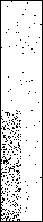
\includegraphics[width=0.1\linewidth]{input-single.png}
	\caption[NS]{
		یک نمونه طرح شطرنجی فعالیت یک الگو به طول ۲۰ واحد زمان که در ادامه‌ی آن نیز ۲۰ واحد زمان هیچ الگویی نمایش داده نشده است.
	}
	\label{fig:input-single} 
\end{figure}
	
	در طول زمان تعین این موضوع که کدام الگو نمایش داده شود به صورت تصادفی و با احتمال یکسان اتفاق می‌افتد. طرح شطرنجی فعالیت یک جمعیت ورودی در یک بازه‌ی زمانی در شکل \ref{fig:input-range} قابل رویت است.
	
\begin{figure}[H]
	\centering
	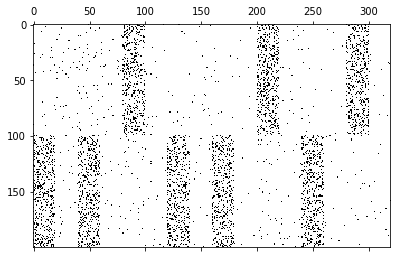
\includegraphics[width=1.0\linewidth]{input-range.png}
	\caption[NS]{
		یک نمونه طرح شطرنجی فعالیت یک جمعیت با ۲۰۰ نورون برای ۳۲۰ واحد زمان که هر الگو برای مدت ۲۰ واحد زمان فعال است و پس از آن برای ۲۰ واحد زمان هیچ الگویی نمایش داده نمی‌شود.
	}
	\label{fig:input-range} 
\end{figure}
	
	\subsection{مدل‌سازی ستون‌های کورتکسی}
	
	برای سادگی در مدل‌سازی ستون‌های کورتکسی به صورت ساختارهایی دو لایه که یک لایه به عنوان لایه‌ی ۴ و لایه‌ی دیگر نیز به عنوان لایه‌‌های ۲ و ۳ در نئوکورتکس در نظر گرفته شده‌اند. در هریک از لایه‌های ستون‌های کورتکسی دو جمعیت برای بازنمایی دو دسته‌از نورون‌های فعال برای دو الگوی فعالیت ممکن در نظر گرفته شده است. بین هر دو جمعیت حاضر در هر لایه یک اتصال مهاری وجود دارد؛ به این صورت که ضربه زدن هر نورون باعث یک اثر مهاری روی مجموعه‌ای از نورون‌ها در جمعیت دیگر می‌شود که وجود این اتصال در عمل نقش حضور \gls{inh} را برای ما ایفا می‌کنند.
	
	در این مدل جریان اطلاعات از لایه‌ی ۴ به سمت لایه‌ی‌ ۲/۳ است که تلاش می‌شود تا در لایه‌ی ۲/۳ یک بازنمایی پایدار‌تر نسبت به لایه‌ی ۴ شکل بگیرد. از این رو یک اتصال پولینگ\LTRfootnote{Pooling} هر جمعیت لایه‌ی ۴ را به جمعیت متناظر خودش در لایه‌ی ۲/۳ متصل می‌کند؛ به این صورت که هر نورون در لایه‌ی ۲/۳ دقیقا از تعداد مشخصی از نورون‌های لایه‌ی ۴ ورودی دریافت می‌کند و هر نورون در لایه‌ی ۴ تنها به یک نورون در لایه‌ی ۲/۳ متصل است. همچنین وزن این اتصالات به گونه‌ای است که فعالیت حتی یک نورون پیش‌سیناپسی نیز در صورت عدم وجود هیچ‌گونه اثر مهاری، باعث گذر از آستانه و شکل گرفتن ضربه در لایه‌ی ۲/۳ می‌شود. 
	
	همچنین در این مدل مجموعه‌ای از اتصالات رو به عقب\LTRfootnote{Backward Connections} نیز در نظر گرفته شده است که وظایف اتصالاتی را بازی می‌کنند که وظیفه‌ی آماده کردن نورون‌های پست سیناپتیک برای ضربه زدن را دارند و وزن این دسته از اتصالات مشخص کننده‌ی میزان درصد نزدیک شدن اختلاف پتانسیل نورون پس‌سیناپسی به آستانه است. به عبارتی نورون‌های پس‌سیناپسی را به آستانه‌ی ضربه نزدیک می‌کنند ولی باعث فعال شدن آن‌ها نمی‌شوند. همچنین دسته‌ی دیگری نیز از اتصالات رو به عقب تعریف شده اند که مشابه مورد قبل هستند ولی نقش مهاری دارند و با فعال شدن نورون‌های پیش‌سیناپسی، اون دسته از اتصالات به همان نسبت اختلاف پتانسیل را به میزان اختلاف پتانسیل حالت استراحت نورون نزدیک‌تر می‌کنند.
	
	شمای کلی مدل پیشنهادی برای هر ستون کورتکسی در شکل \ref{fig:model_cc} قابل مشاهده است. 
	
	\begin{figure}[]
		\centering
		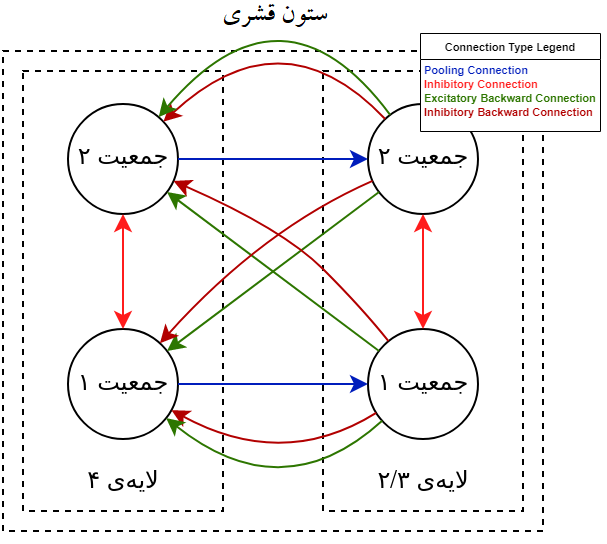
\includegraphics[width=1.0\linewidth]{model_cc.png}
		\caption[NS]{
			شمای کلی مدل پیشنهادی برای ستون کورتکسی که در آن جمعیت‌ها و اتصالات بین آن‌ها مشخص شده‌اند. جهات پیکان‌ها مشخص کننده‌ی جمعیت پس‌سیناپسی است و رنگ پیکان‌ها مشخص کننده‌ی نوع اتصالات هستند. پیکان آپی نمایان‌گر اتصال پولینگ، قرمز روشن نمایان‌گر اتصال مهاری، سبز نمایان‌گر اتصالات رو به عقب تحریکی و نهایتا اتصالات با رنگ قرمز تیره مشخص کننده‌ی اتصالات رو به عقب مهاری هستند.
		}
		\label{fig:model_cc} 
	\end{figure}
	
	
	\subsection{اتصالات پیش‌خور بین ستون‌های کورتکسی و جمعیت‌های ورودی}
	
	دو ستون کورتکسی‌ای که جمعیت‌های ورودی به لایه ۴ آن‌ها متصل شده‌اند، باید داده را به ستون کورتکسی دیگر (که پس از این با نام «ستون کورتکسی سوم» به آن اشاره می‌کنیم) منتقل کنند تا اطلاعات در آنجا تجمیع شوند و یک درک واحد از ورودی دو ستون کورتکسی در آنجا شکل بگیرد. برای این منظور لایه‌ی ۲/۳ این دو ستون کورتکسی با یک اتصال تحریکی به لایه ۴ ستون کورتکسی سوم متصل می‌شوند. به عبارتی هرکدام از جمعیت‌های نورونی موجود در لایه‌ی ۲/۳ هر کدام از ستون‌های کورتکسی اول و دوم یک اتصال تحریکی به هر‌یک از جمعیت‌های نورونی لایه‌ی ۴ ستون کورتکسی سوم دارند. 
	
	همچنین از جمعیت‌های ورودی نیز یک اتصال تحریکی به جمعیت‌های حاضر در لایه‌ی ۴ ستون ‌های کورتکسی در نظر گرفته شده تا فعالیت ورودی‌ها به ستون‌های کورتکسی منتقل شوند.
	
	\subsection{اتصالات رو‌ به عقب بین ستون‌های کورتکسی}
	
	مشابه اتصالات رو به عقبی که در داخل هر ستون کورتکسی تعریف شده بودند، اتصالاتی بین جمعیت‌های دو ستون کورتکسی نیز تعریف می‌شوند که نقش اتصالات از راه دور حاضر در مغز را برای ما ایفا می‌کنند. ساختار این اتصالات به این صورت است که اتصالات از لایه‌ی ۲/۳ ستون کورتکسی سوم به لایه‌های ۲/۳ ستون‌های کورتکسی اول و دوم هم اتصالات رو به عقب تحریکی و هم اتصالات رو به عقب مهاری وجود دارند و مکانیزم این اتصالات رو به عقب مشابه با اتصالات رو به عقبی است که در داخل ستون‌های کورتکسی تعریف شده بودند.
	
	شمای کلی مدل پیشنهاد شده در شکل \ref{fig:model_overall} قابل رؤیت است.
	
	\begin{figure}[]
		\centering
		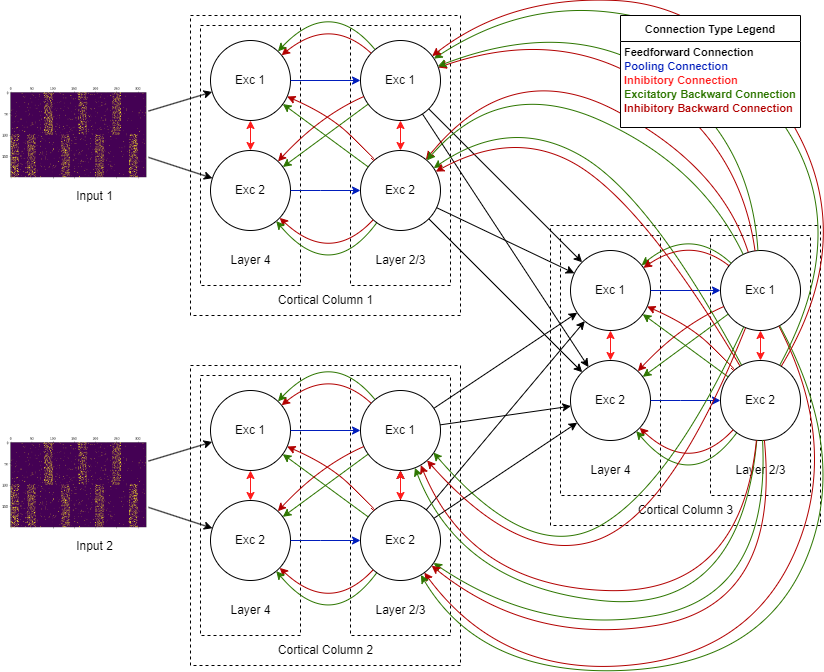
\includegraphics[width=1.0\linewidth]{model_overall.png}
		\caption[NS]{
			مدل پیشنهادی که در آن تمام جمعیت‌ها و اتصالات بین آن‌ها مشخص شده است. همچنین رنگ اتصالات نیز مشابه با رنگ اتصالات تعریف شده در شکل \ref{fig:model_cc} می‌باشد.
		}
		\label{fig:model_overall} 
	\end{figure}

	\subsection{وزن‌های اولیه و انعطاف پذیری نورونی}
	نرخ اتصالات بین هر دو جمعیت در مدل به صورت از پیش تعریف شده و ثابت می‌باشد. به این صورت که تعدادی از اتصالات بین دو جمعیت در ابتدای مدل‌سازی به صورت تصادفی با احتمال از پیش تعین شده، انتخاب و کاملا حذف می‌شوند که برای این منظور وزنشان برای تمام طول شبیه‌سازی صفر در نظر گرفته می‌شود.
	
	برای مقداردهی اولیه‌ی وزن‌های تمام اتصالات، بجز اتصالات رو به عقب، از توزیع یکنواخت در بازه‌ی مشخص شده برای هر جمعیت استفاده شده است و برای مقداردهی اولیه‌ی وزن‌های اتصالات رو به عقب نیز از توزیع بتا\LTRfootnote{Beta Distribution} استفاده شده است. همانطور که پیش‌تر نیز اشاره شده بود سازوکار اتصالات رو به عقب به گونه ای است که وزن آن‌ها بیانگر درصد تاثیرگذاری آن‌ها است و به همین دلیل مقادیر همواره در بازه‌ی صفر و یک هستند.
	
	\begin{figure}[]
		\centering
		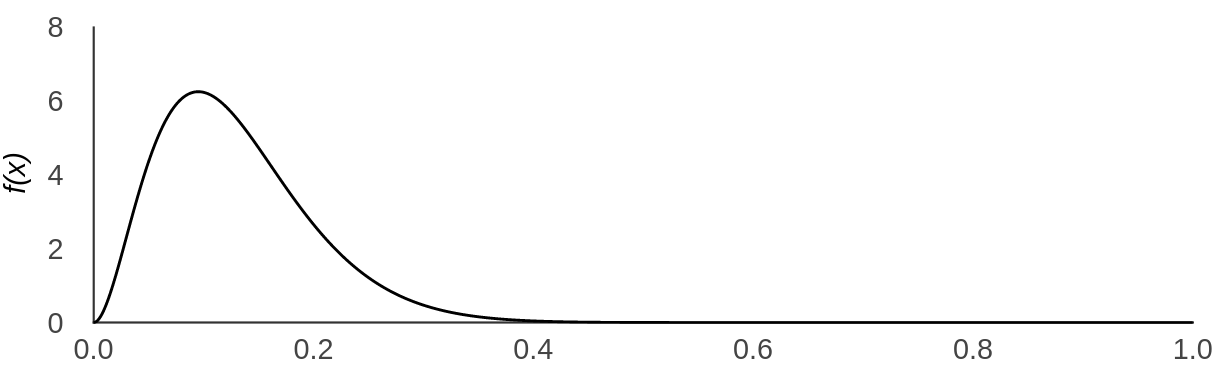
\includegraphics[width=0.8\linewidth]{beta-3-20.png}
		\caption[NS]{
			یک نمونه توزیع بتا با پارامتر‌های $\alpha=3$ و $\beta=20$.
		}
		\label{fig:beta} 
	\end{figure}
	
	همچنین در مدل ارائه شده اتصالات متنوعی بین جمعیت‌های مختلف حاضر در مدل به کار گرفته شده‌اند و روی هریک از آن‌ها نیز می‌توان یک سازوکار برای انعطاف پذیری نورونی و تغیرات وزن اتصالات در طول زمان تعریف کرد. لازم به ذکر است که برای مجموعه‌ی اتصالات مهاری بین جمعیت‌های یک لایه از ستون کورتکسی، انعطاف پذیری نورونی مشخص نشده و وزن اتصالاتشان در تمام طول شبیه‌سازی ثابت هستند. تمام قوانین یادگیری مورد استفاده، قوانین یادگیری تقویتی هستند که به دلیل ساختار ورودی‌ها که الگوی رفتاری جمعیت‌های ورودی برای بازه‌هایی با طول زمان مشخص ثابت هستند، شخصی سازی شده‌اند؛ به این صورت که میزان دوپامین نه در هر لحظه، بلکه در انتهای بازه‌ی نمایش هر الگو محاسبه می‌گردد و در طول بازه‌ی نمایش یک الگو در ورودی، هیچ تغیری توسط قوانین یادگیری روی وزن‌های اتصالات اعمال نمی‌شود و تمام این تغیرات تجمیع شده و نهایتا با توجه به میزان دوپامین محاسبه شده در انتهای هر بازه به صورت یکجا روی اتصالات اعمال می‌شوند. میزان تغیرات وزن در زمان $t$ در فرمول \ref{eq:seasonal} مشخص شده است که در آن $|pattern|$ طول بازه‌ی نمایش هر الگو و $STDP(t')$ نیز میزان تغیرات وزن در صورت اعمال انعطاف پذیری وابسته به زمان ضربه در زمان $t'$ است.
	
	\begin{align}
		\Delta w_t =
		\begin{cases}
			d \times \sum_{t'=t-\left | pattern \right |+1}^{t} STDP(t') & \text{if}~t\bmod\left | pattern \right | = 0\\
			0 & \text{otherwise}
		\end{cases}  
		\label{eq:seasonal}
	\end{align}
	
	میزان دوپامین برای پاداش و تنبیه نیز در هر لحظه بر اساس مقایسه‌ی میزان فعالیت (تعداد ضربه‌ها در طول بازه‌ی نمایش الگو) جمعیت‌های لایه‌ی ۲/۳ ستون کورتکسی سوم محاسبه می‌گردد. به این صورت که هریک از دو الگوی فعالیت که نورون‌های ورودی به خود می‌گیرند، با یکی از دو جمعیت این لایه متناظر می‌شوند و در صورتی که جمعیت متناظر با الگوی در حال نمایش فعالیت بیشتری نسبت به جمعیت دیگر داشته باشد، پاداش و در غیر این صورت تنبیه برای مدل لحاظ می‌شود. همچنین میزان شدت پاداش و تنبیه نیز بر اساس میزان اختلاف فعالیت این دو جمعیت تعیین می‌گردد.
	
	

	\subsection{ابزار‌های پیاده‌سازی}
	
	پیاده‌سازی‌های مربوط با مدل ارائه شده با زبان برنامه نویسی پایتون و بر بستر چارچوب\LTRfootnote{Framework} نرم‌افزاری بایندزنت\LTRfootnote{Bindsnet}، که خود برپایه‌ی چارچوب پای‌تورچ\LTRfootnote{PyTorch} توسعه داده شده است، انجام شده است. از جمله ویژگی‌های مورد نظر که چارچوب نرم‌افزاری بر اساس آن‌ها انتخاب شده است می‌توان به توان پردازش مجاسبات تنسوری توسط پردازنده و کارت گرافیک و از پیش تعریف شدن مدل های نورونی پایه، همچون مدل نورونی تجمیع و آتش، انعطاف پذیری نورونی و محاسبات مربوط به اتصالات بین نورون‌ها، اشاره کرد.
	
	همچنین به دلیل نیاز به مجموعه‌ای از سازوکار‌ها و ساختارهایی که در هیچ یک از چارچوب‌های مورد‌استفاده از پیش تعریف نشده بودند، یک چارچوب نرم‌افزاری بر بستر بایندزنت توسعه داده شده است که در عمل مدل‌سازی های نهایی بر بستر آن انجام شده اند.
	
	\subsection{پارامتر‌های مورد استفاده در آزمایش}
	اجزای مختلف مدل ارائه شده پارامتر‌های مختلفی دارند که در نتیجه‌ی آزمایش تاثیر بسیار مهمی دارند. مواردی همچون تعداد نورون‌های جمعیت‌های مختلف، نرخ‌های یادگیری، نرخ اتصالات بین جمعیت ها و بسیاری موارد دیگر. همچنین با توجه به پیچیدگی مدل و پیچیدگی سیستم حاصل از پیاده سازی آن با استفاده از شبکه‌های عصبی ضربه‌ای، تنظیم کردن این پارامتر‌ها به گونه‌ای که شبکه عملکرد مناسبی داشته باشد موضوعی بسیار چالش برانگیز است. پارامتر‌های مورد استفاده برای آزمایش در سه جدول \ref{table:parameters-cc-3}، \ref{table:parameters-cc-1-2} و \ref{table:parameters-details} مشخص شده‌اند.

\begin{table}[p]
	\centering
	\resizebox{\textwidth}{!}{
	\begin{tabular}{|rrrl|}
		\hline
		\multicolumn{4}{|c|}{\textbf{ستون‌های کورتکسی اول و دوم}}                                                                                                                                                              \\ \hline
		\multicolumn{1}{|r|}{\multirow{8}{*}{لایه ۴}}                   & \multicolumn{1}{r|}{\multirow{6}{*}{جمعیت ها}}                 & \multicolumn{1}{r|}{تعداد نورون‌های هر جمعیت}             & $100$                     \\ \cline{3-4} 
		\multicolumn{1}{|r|}{}                                          & \multicolumn{1}{r|}{}                                          & \multicolumn{1}{r|}{اثر ثابت زمانی\LTRfootnote{Time Constant Trace}} & $6$                       \\ \cline{3-4} 
		\multicolumn{1}{|r|}{}                                          & \multicolumn{1}{r|}{}                                          & \multicolumn{1}{r|}{آستانه‌ی ضربه}                        & $-52$                     \\ \cline{3-4} 
		\multicolumn{1}{|r|}{}                                          & \multicolumn{1}{r|}{}                                          & \multicolumn{1}{r|}{ولتاژ استراحت}                        & $-65$                     \\ \cline{3-4} 
		\multicolumn{1}{|r|}{}                                          & \multicolumn{1}{r|}{}                                          & \multicolumn{1}{r|}{بازه‌ی عدم فعالیت پس از ضربه}         & $3$                       \\ \cline{3-4} 
		\multicolumn{1}{|r|}{}                                          & \multicolumn{1}{r|}{}                                          & \multicolumn{1}{r|}{ثابت زمانی کاهش}                      & $10$                      \\ \cline{2-4} 
		\multicolumn{1}{|r|}{}                                          & \multicolumn{1}{r|}{\multirow{2}{*}{اتصال مهاری بین دو جمعیت}} & \multicolumn{1}{r|}{بازه‌ی وزن}                           & $(-0.4,0)$                \\ \cline{3-4} 
		\multicolumn{1}{|r|}{}                                          & \multicolumn{1}{r|}{}                                          & \multicolumn{1}{r|}{نرخ اتصال}                            & $0.3$                     \\ \hline
		\multicolumn{1}{|r|}{\multirow{8}{*}{\textbf{لایه ۲/۳}}}        & \multicolumn{1}{r|}{\multirow{6}{*}{جمعیت ها}}                 & \multicolumn{1}{r|}{تعداد نورون‌های هر جمعیت}             & $32$ \\ \cline{3-4} 
		\multicolumn{1}{|r|}{}                                          & \multicolumn{1}{r|}{}                                          & \multicolumn{1}{r|}{اثر ثابت زمانی} & $10$                      \\ \cline{3-4} 
		\multicolumn{1}{|r|}{}                                          & \multicolumn{1}{r|}{}                                          & \multicolumn{1}{r|}{آستانه‌ی ضربه}                        & $-52$                     \\ \cline{3-4} 
		\multicolumn{1}{|r|}{}                                          & \multicolumn{1}{r|}{}                                          & \multicolumn{1}{r|}{ولتاژ استراحت}                        & $-65$                     \\ \cline{3-4} 
		\multicolumn{1}{|r|}{}                                          & \multicolumn{1}{r|}{}                                          & \multicolumn{1}{r|}{بازه‌ی عدم فعالیت پس از ضربه}         & $3$                       \\ \cline{3-4} 
		\multicolumn{1}{|r|}{}                                          & \multicolumn{1}{r|}{}                                          & \multicolumn{1}{r|}{ثابت زمانی کاهش}                      & $10$                      \\ \cline{2-4} 
		\multicolumn{1}{|r|}{}                                          & \multicolumn{1}{r|}{\multirow{2}{*}{اتصال مهاری بین دو جمعیت}} & \multicolumn{1}{r|}{بازه‌ی وزن}                           & $(-0.4,0)$                \\ \cline{3-4} 
		\multicolumn{1}{|r|}{}                                          & \multicolumn{1}{r|}{}                                          & \multicolumn{1}{r|}{نرخ اتصال}                            & $1.0$                     \\ \hline
		\multicolumn{1}{|r|}{\multirow{3}{*}{اتصال پولینگ بین دو لایه}} & \multicolumn{2}{r|}{اندازه‌ی کرنل}                                                                                         & $5$                       \\ \cline{2-4} 
		\multicolumn{1}{|r|}{}                                          & \multicolumn{2}{r|}{وزن اتصال}                                                                                             & $14$                      \\ \cline{2-4} 
		\multicolumn{1}{|r|}{}                                          & \multicolumn{2}{r|}{اندازه‌ی گام}                                                                                          & $3$                       \\ \hline
		\multicolumn{1}{|r|}{\multirow{6}{*}{اتصالات رو به عقب}}        & \multicolumn{2}{r|}{پارامتر‌های توزیع بتا}                                                                                 & $\alpha=3, \beta=40$               \\ \cline{2-4} 
		\multicolumn{1}{|r|}{}                                          & \multicolumn{2}{r|}{نرخ اتصال}                                                                                             & $0.2$                     \\ \cline{2-4} 
		\multicolumn{1}{|r|}{}                                          & \multicolumn{2}{r|}{بازه‌ی وزن}                                                                                            & $(0, 0.95)$               \\ \cline{2-4} 
		\multicolumn{1}{|r|}{}                                          & \multicolumn{2}{r|}{نرخ یادگیری}                                                                                           & $0.003 - 0.008$           \\ \cline{2-4} 
		\multicolumn{1}{|r|}{}                                          & \multicolumn{2}{r|}{وزن کاهش}                                                                                              & $0.00005$                \\ \cline{2-4} 
		\multicolumn{1}{|r|}{}                                          & \multicolumn{2}{r|}{ثابت زمانی}                                                                                            & $6$                       \\ \hline
	\end{tabular}}
\caption{\label{table:parameters-cc-1-2}پارامتر‌های مربوط به ستون‌های کورتکسی اول و دوم}
\end{table}


\begin{table}[p]
	\centering
	\resizebox{\textwidth}{!}{
		\begin{tabular}{|rrrl|}

\hline
\multicolumn{4}{|c|}{\textbf{ستون‌ کورتکسی سوم}}                                                                                                                                                               \\ \hline
\multicolumn{1}{|r|}{\multirow{8}{*}{لایه ۴}}                   & \multicolumn{1}{r|}{\multirow{6}{*}{جمعیت ها}}                 & \multicolumn{1}{r|}{تعداد نورون‌های هر جمعیت}     & $100$                     \\ \cline{3-4} 
\multicolumn{1}{|r|}{}                                          & \multicolumn{1}{r|}{}                                          & \multicolumn{1}{r|}{اثر ثابت زمانی}               & $6$                       \\ \cline{3-4} 
\multicolumn{1}{|r|}{}                                          & \multicolumn{1}{r|}{}                                          & \multicolumn{1}{r|}{آستانه‌ی ضربه}                & $-52$                     \\ \cline{3-4} 
\multicolumn{1}{|r|}{}                                          & \multicolumn{1}{r|}{}                                          & \multicolumn{1}{r|}{ولتاژ استراحت}                & $-65$                     \\ \cline{3-4} 
\multicolumn{1}{|r|}{}                                          & \multicolumn{1}{r|}{}                                          & \multicolumn{1}{r|}{بازه‌ی عدم فعالیت پس از ضربه} & $3$                       \\ \cline{3-4} 
\multicolumn{1}{|r|}{}                                          & \multicolumn{1}{r|}{}                                          & \multicolumn{1}{r|}{ثابت زمانی کاهش}              & $10$                      \\ \cline{2-4} 
\multicolumn{1}{|r|}{}                                          & \multicolumn{1}{r|}{\multirow{2}{*}{اتصال مهاری بین دو جمعیت}} & \multicolumn{1}{r|}{بازه‌ی وزن}                   & $(-0.3,0)$                \\ \cline{3-4} 
\multicolumn{1}{|r|}{}                                          & \multicolumn{1}{r|}{}                                          & \multicolumn{1}{r|}{نرخ اتصال}                    & $0.3$                     \\ \hline
\multicolumn{1}{|r|}{\multirow{8}{*}{لایه ۲/۳}}                 & \multicolumn{1}{r|}{\multirow{6}{*}{جمعیت ها}}                 & \multicolumn{1}{r|}{تعداد نورون‌های هر جمعیت}     & $32$ \\ \cline{3-4} 
\multicolumn{1}{|r|}{}                                          & \multicolumn{1}{r|}{}                                          & \multicolumn{1}{r|}{اثر ثابت زمانی}               & $10$                      \\ \cline{3-4} 
\multicolumn{1}{|r|}{}                                          & \multicolumn{1}{r|}{}                                          & \multicolumn{1}{r|}{آستانه‌ی ضربه}                & $-52$                     \\ \cline{3-4} 
\multicolumn{1}{|r|}{}                                          & \multicolumn{1}{r|}{}                                          & \multicolumn{1}{r|}{ولتاژ استراحت}                & $-65$                     \\ \cline{3-4} 
\multicolumn{1}{|r|}{}                                          & \multicolumn{1}{r|}{}                                          & \multicolumn{1}{r|}{بازه‌ی عدم فعالیت پس از ضربه} & $3$                       \\ \cline{3-4} 
\multicolumn{1}{|r|}{}                                          & \multicolumn{1}{r|}{}                                          & \multicolumn{1}{r|}{ثابت زمانی کاهش}              & $10$                      \\ \cline{2-4} 
\multicolumn{1}{|r|}{}                                          & \multicolumn{1}{r|}{\multirow{2}{*}{اتصال مهاری بین دو جمعیت}} & \multicolumn{1}{r|}{بازه‌ی وزن}                   & $(-0.3,0)$                \\ \cline{3-4} 
\multicolumn{1}{|r|}{}                                          & \multicolumn{1}{r|}{}                                          & \multicolumn{1}{r|}{نرخ اتصال}                    & $1.0$                     \\ \hline
\multicolumn{1}{|r|}{\multirow{3}{*}{اتصال پولینگ بین دو لایه}} & \multicolumn{2}{r|}{اندازه‌ی کرنل}                                                                                 & $5$                       \\ \cline{2-4} 
\multicolumn{1}{|r|}{}                                          & \multicolumn{2}{r|}{وزن اتصال}                                                                                     & $14$                      \\ \cline{2-4} 
\multicolumn{1}{|r|}{}                                          & \multicolumn{2}{r|}{اندازه‌ی گام}                                                                                  & $3$                       \\ \hline
\multicolumn{1}{|r|}{\multirow{6}{*}{اتصالات رو به عقب}}        & \multicolumn{2}{r|}{پارامتر‌های توزیع بتا}                                                                         & $\alpha=3, \beta=80$               \\ \cline{2-4} 
\multicolumn{1}{|r|}{}                                          & \multicolumn{2}{r|}{نرخ اتصال}                                                                                     & $0.2$                     \\ \cline{2-4} 
\multicolumn{1}{|r|}{}                                          & \multicolumn{2}{r|}{بازه‌ی وزن}                                                                                    & $(0, 0.95)$               \\ \cline{2-4} 
\multicolumn{1}{|r|}{}                                          & \multicolumn{2}{r|}{نرخ یادگیری}                                                                                   &    $0.003 - 0.007$        \\ \cline{2-4} 
\multicolumn{1}{|r|}{}                                          & \multicolumn{2}{r|}{وزن کاهش}                                                                                      & $0.00005$                \\ \cline{2-4} 
\multicolumn{1}{|r|}{}                                          & \multicolumn{2}{r|}{ثابت زمانی}                                                                                    & $6$                       \\ \hline
	\end{tabular}}
\caption{\label{table:parameters-cc-3}پارامتر‌های مربوط به ستون‌ کورتکسی سوم}
\end{table}


\begin{table}[p]
\centering
\resizebox{0.95\textwidth}{!}{
	\begin{tabular}{|rrrl|}
		\hline
		\multicolumn{4}{|c|}{\textbf{جمعیت‌های ورودی}}                                                                  \\ \hline
		\multicolumn{3}{|r|}{تعداد نورون‌ها}                                                      & $200$                 \\ \hline
		\multicolumn{3}{|r|}{اثر ثابت زمانی}                                & $6$                   \\ \hline
		\multicolumn{4}{|c|}{\textbf{اتصالات جمعیت ورودی به ستون‌های کورتکسی}}                                          \\ \hline
		\multicolumn{3}{|r|}{بازه‌ی وزن}                                                          & $(0, 0.5)$            \\ \hline
		\multicolumn{3}{|r|}{نرخ یادگیری مثبت}                                                    & $0.01$                \\ \hline
		\multicolumn{3}{|r|}{نرخ یادگیری منفی}                                                    & $0.02$               \\ \hline
		\multicolumn{3}{|r|}{نرخ اتصال}                                                           & $0.3$                 \\ \hline
		\multicolumn{3}{|r|}{ثابت زمانی}                                                          & $6$                   \\ \hline
		\multicolumn{4}{|c|}{\textbf{الگو‌های فعالیت ورودی}}                                                            \\ \hline
		\multicolumn{3}{|r|}{زمان نمایش هر الگو}                                                  & $20$                  \\ \hline
		\multicolumn{3}{|r|}{زمان استراحت (بدون نمایش الگو پس از هر نمایش الگو)}                  & $20$                  \\ \hline
		\multicolumn{3}{|r|}{احتمال فعالیت نورون‌ها در زمان استراحت}                              & $0.01\pm 0.005$        \\ \hline
		\multicolumn{3}{|r|}{احتمال فعالیت نورون‌ها در زمان نمایش الگو}                           & $\sim 0.2$           \\ \hline
		\multicolumn{4}{|c|}{\textbf{اتصالات رو به عقب بین ستون‌های کورتکسی}}                                           \\ \hline
		\multicolumn{3}{|r|}{پارامتر‌های توزیع بتا}                                               & $\alpha=3, \beta=80$           \\ \hline
		\multicolumn{3}{|r|}{نرخ اتصال}                                                           & $0.2$                 \\ \hline
		\multicolumn{3}{|r|}{بازه‌ی وزن}                                                          & $(0, 0.95)$           \\ \hline
		\multicolumn{3}{|r|}{نرخ یادگیری}                                                         & $0.003 - 0.007$       \\ \hline
		\multicolumn{3}{|r|}{وزن کاهش}                                                            & $0.00005$             \\ \hline
		\multicolumn{3}{|r|}{ثابت زمانی}                                                          & $6$                   \\ \hline
		\multicolumn{4}{|c|}{\textbf{زمان‌های آموزش}}                                                                   \\ \hline
		\multicolumn{3}{|r|}{تعداد الگو‌های نمایش داده شده برای آموزش ستون‌های کورتکسی اول و دوم} & $800$                \\ \hline
		\multicolumn{3}{|r|}{تعداد الگو‌های نمایش داده شده در گام اول همراه با اتصالات رو به عقب} & $200$                \\ \hline
		\multicolumn{3}{|r|}{تعداد الگو‌های نمایش داده شده برای آموزش ستون کورتکسی سوم}           & $500$                 \\ \hline
\end{tabular}}
\caption{\label{table:parameters-details}پارامتر‌های جزئی مربوط به مدل مورد استفاده}
\end{table}





	
	\section{آموزش}
	برای رسیدن به نتیجه‌ی نهایی که شکل گیری انقیاد در مدل طراحی شده است لازم است تا مدل آموزش داده شود تا وزن‌های سیناپسی متناسب با داده‌های ورودی تنظیم شوند. 
	فرآیند آموزش دادن مدل شامل سه مرحله‌ی اصلی خواهد بود:
	
	\begin{itemize}
		\item آموزش دادن ستون کورتکسی متناظر با اولین جمعیت ورودی و اتصالات بین جمعیت ورودی و ستون کورتکسی.
		\item آموزش دادن ستون کورتکسی متناظر با دومین جمعیت ورودی و اتصالات بین جمعیت ورودی و ستون کورتکسی.
		\item آموزش دادن اتصالاتی که در آن‌ها ستون کورتکسی سوم دخیل است با استفاده از دو ستون کورتکسی آموزش داده شده.
	\end{itemize}

	در گام اول برای آموزش ستون‌های کورتکسی متناظر با جمعیت‌های ورودی (دو مرحله‌ی اول آموزش) شبکه‌ای به صورت محدود شامل جمعیت ورودی و ستون کورتکسی متناظر، بدون اتصالات رو به عقب در نظر گرفته می‌شود و برای مدت زمان مشخصی شبکه اجرا می‌شود. با توجه به عدم حضور ستون کورتکسی سوم در این شبکه میزان دوپامین در این شبکه، با سازوکاری مشابه با مدل اصلی، توسط لایه ۲/۳ ستون کورتکسی حاضر محاسبه می‌شود. سپس به این شبکه اتصالات رو به عقب همان ستون کورتکسی نیز اضافه می‌شود و مجددا برای زمانی کوتاه‌تر از زمان اجرای پیشین، یادگیری شبکه در مجاورت ورودی ادامه پیدا می‌کند.
	
	در گام بعدی وزن‌های حاصل شده از آموزش دو مدل آموزش داده شده در مدل اصلی جایگزین می‌شوند و یادگیری روی این دسته از سیناپس‌ها متوقف می‌شود. سپس مجددا شبکه برای مدت زمان مشخصی اجرا می‌شود تا وزن‌های سیناپسی مربوط به اتصالات بین مدل‌های قبلی و ستون کورتکسی سوم نیز آموزش داده شوند.
	

	\section{نتایج}
	پس از این‌که مدل آموزش داده‌شد، وزن‌های اتصالات بین جمعیت‌ها که در ابتدا به صورت تصادفی توزیع شده بودند، تغیر کرده اند. با توجه به این‌که آموزش در دو گام کلی رخ داده بود، نتایج این آزمایش نیز در دو بخش مربوط به نتایج آموزش ستون‌های کورتکسی اول و دوم، که ستون‌های متصل به ورودی بودند، و ستون کورتکسی سوم، که حاصل تجمیع اطلاعات دو ستون کورتکسی پیشین بود، گزارش می‌گردد.
	
	برای سادگی، در این گزارش، تنها نتایج مربوط به یک آزمایش بخصوص گزارش شده است، ولی فرآیند آموزش و نتایج آن کاملا تکرار پذیر هستند و منحصر به تلاش‌های خاصی نمی‌شوند.
	
	همچنین در ادامه‌ی فصل به مشخص کردن میزان پیشرفت یادگیری و نهایتا گزارش دقت نهایی مدل در تلاش ها‌ی مختلف اشاره خواهیم کرد.
	
	\subsection{نتایج آموزش ستون‌های کورتکسی اول و دوم}
	طبیعتا در ابتدای فرآیند آموزش، الگوی رفتاری مدل شکلی تصادفی دارد و بین الگوی نمایش داده شده در جمعیت‌های ورودی و الگوی رفتاری جمعیت‌های لایه‌ی ۲/۳ ستون کورتکسی، هم‌بستگی بسیار کمی وجود دارد. یک نمونه فعالیت جمعیت‌های لایه‌ ۲/۳ ستون کورتکسی در 400 میلی‌ثانیه‌ی اول شبیه‌سازی در تصویر ‌\ref{fig:c1-begining} قابل مشاهده است.
	
	\begin{figure}[H]
		\centering
		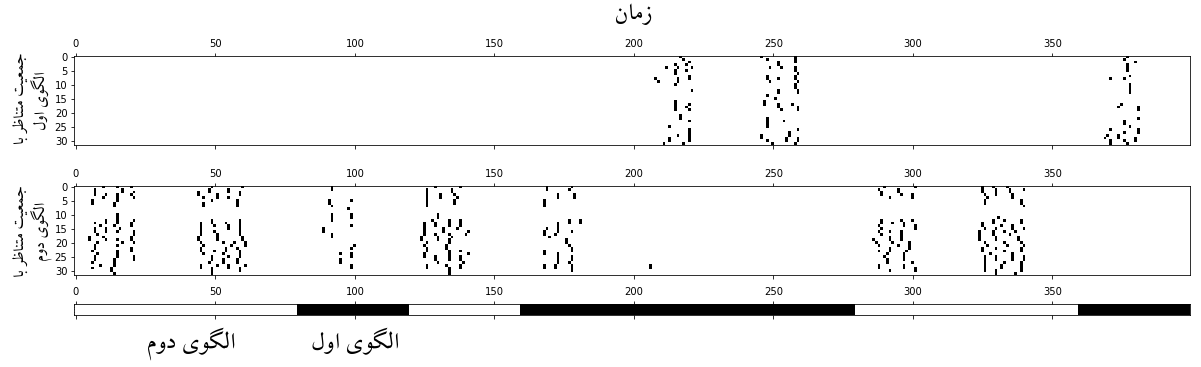
\includegraphics[width=1.0\linewidth]{c1-begining.png}
		\caption[NS]{
			نمایش شطرنجی فعالیت نورون‌های جمعیت‌های لایه‌ی ۲/۳ ستون کورتکسی در ۴۰۰ میلی‌ثانیه‌ی ابتدایی که در تصویر فوق، سطر اول فعالیت جمعیت نورونی متناظر با الگوی اول، سطر دوم جمعیت متناظر با الگوی دوم و نوار نمایش داده در سطر سوم نیز نمایش دهنده‌ی الگوی نشان داده شده در ورودی در آن زمان است که رنگ مشکی نشان‌ دهنده‌ی نمایش الگوی اول در ورودی و رنگ سفید نشان دهنده‌ی نمایش الگوی دوم در ورودی است.
		}
		\label{fig:c1-begining} 
	\end{figure}
	
	با گذر زمان و پیشرفت فرآیند یادگیری هم‌بستگی بین ورودی و لایه‌ی ۲/۳ افزایش پیدا می‌کند؛ به طوری که فعالیت هر جمعیت از لایه‌ی ۲/۳ وابسته به نمایش الگوی متناظر با آن در جمعیت‌های ورودی می‌شود. یک نمونه فعالیت جمعیت‌های ستون کورتکسی لایه‌ ۲/۳ در بازه‌ی زمانی میلی‌ثانیه‌ی ۳۹۶۰۰ تا میلی‌ثانیه‌ی ۴۰۰۰۰ (نمایش ۱۰ الگوی انتهایی) در تصویر \ref{fig:c1-final} نمایش داده شده است که افزایش هم‌بستگی در آن به وضوح قابل مشاهده است.
	
	\begin{figure}[H]
		\centering
		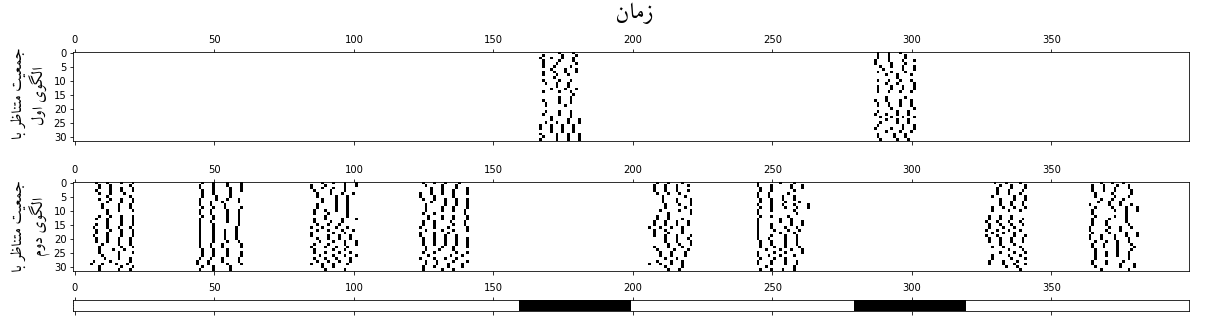
\includegraphics[width=1.0\linewidth]{c1-final.png}
		\caption[NS]{
			نمایش شطرنجی فعالیت نورون‌های جمعیت‌های لایه‌ی ۲/۳ ستون کورتکسی در بازه‌ی میلی‌ثانیه‌ی ۳۹۶۰۰ و میلی‌ثانیه‌ی ۴۰۰۰۰ که در تصویر فوق، مشابه با تصویر \ref{fig:c1-begining} سطر اول فعالیت جمعیت نورونی متناظر با الگوی اول، سطر دوم جمعیت متناظر با الگوی دوم و نوار نمایش داده در سطر سوم نیز نمایش دهنده‌ی الگوی نشان داده شده در ورودی در آن زمان است که رنگ مشکی نشان‌ دهنده‌ی نمایش الگوی اول در ورودی و رنگ سفید نشان دهنده‌ی نمایش الگوی دوم در ورودی است.
		}
		\label{fig:c1-final} 
	\end{figure}
	
	\subsection{نتایج آموزش ستون کورتکسی سوم}
	
	همانطور که در بخش قبل‌نیز به آن اشاره شد، پس از آموزش ستون‌های کورتکسی متصل به ورودی، آن‌ها را به یک ستون کورتکسی سوم متصل می‌کنیم و اتصالات بین آن‌ها را نیز برقرار می‌کنیم و مجددا شبکه را آموزش می‌دهیم. در ابتدای این موضوع رفتار ستون کورتکسی سوم بسیار نا دقیق است ولی به مرور زمان رفتار نورون‌های حاضر در مدل به سمتی متمایل می‌شود که هم‌بستگی بین ورودی و رفتار جمعیت‌های لایه‌ی ۲/۳ ستون کورتکسی سوم بسیار افزایش پیدا می‌کند. الگوی رفتاری جمعیت‌های لایه‌ی ۲/۳ ستون کورتکسی سوم در ابتدا و انتهای بازه‌ی آموزش، به ترتیب در تصاویر ‌\ref{fig:c3-begining} و \ref{fig:c3-final} قابل مشاهده است.
	
	\begin{figure}[H]
		\centering
		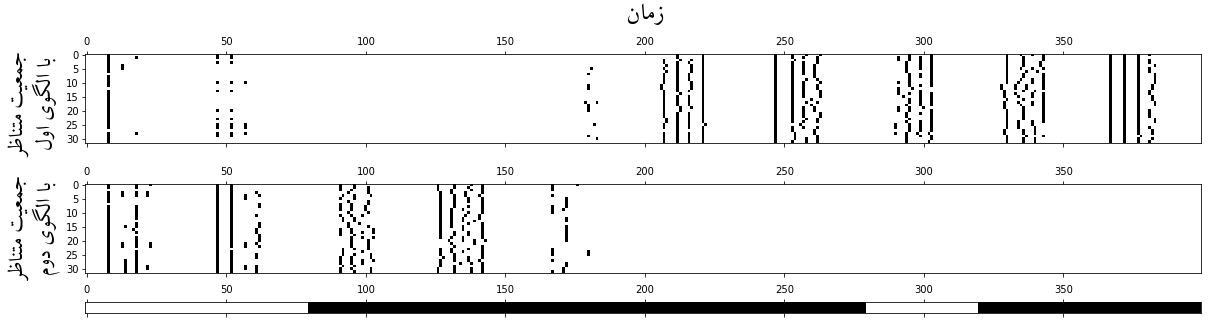
\includegraphics[width=1.0\linewidth]{c3-begining.png}
		\caption[NS]{
			فعالیت لایه‌ی ۲/۳ ستون کورتکسی سوم در ۴۰۰ میلی‌ثانیه‌ی ابتدایی از آموزش ستون کورتکسی سوم.
		}
		\label{fig:c3-begining} 
	\end{figure}

\begin{figure}[H]
	\centering
	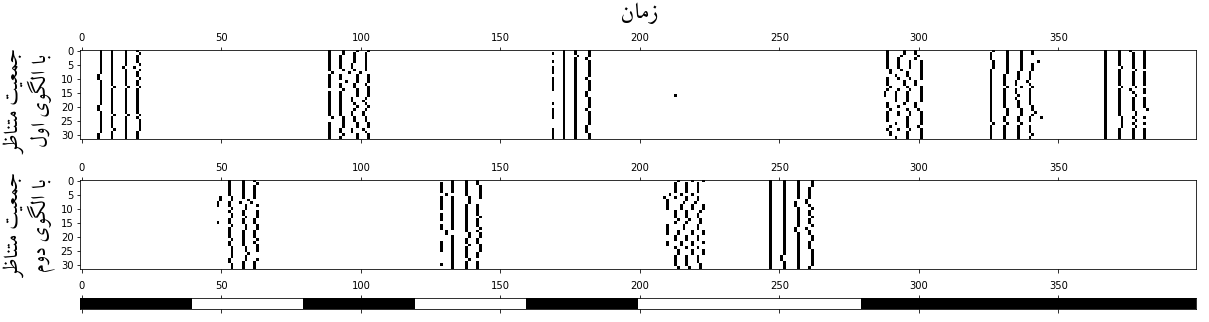
\includegraphics[width=1.0\linewidth]{c3-final.png}
	\caption[NS]{
	فعالیت لایه‌ی ۲/۳ ستون کورتکسی سوم در ۴۰۰ میلی‌ثانیه‌ی انتهایی از آموزش ستون کورتکسی سوم.
	}
	\label{fig:c3-final} 
\end{figure}
	
	\subsection{میزان پیشرفت یادگیری}
	
	در طول آموزش انتظار می‌رود وزن نورون‌های هر یک از اتصالات نورونی به یکی از مقادیر مینیمم و ماکزیمم وزنش همگرا شود. بر همین اساس یک مقدار همگرایی تعریف می‌شود که می‌توان با آن میزان پیشرفت یادگیری را اندازه‌گیری کرد. این معیار همگرایی برای سیناپس $i$ با وزن $w_i$ به صورت زیر تعریف می‌شود که همواره عددی بین صفر و یک می‌باشد:
	
	\begin{align}
		convergence_i = \frac{2 (w_i - w_{min})(w_{max} - w_i) }{ w_{max} - w_{min} }
		\label{eq:convergence_single}
	\end{align}

	به هر میزان که وزن به کمینه و بیشینه‌ی خود نزدیکتر باشد مقدار رابطه‌ی فوق نیز به صفر نزدیکتر می‌شود و بیشینه‌ی آن نیز در حالتی است که وزن نورون دقیقا در نقطه‌ی میانگین کمینه و بیشینه قرار داشته باشد. همچنین از رابطه‌ی فوق می‌توان این معیار را برای یک مجموعه از سیناپس‌ها مثل $S$ به صورت زیر محاسبه کرد:
	
	\begin{align}
		convergence_{S} = \sum_{i \in S} \frac{convergence_i}{|S|} 
		\label{eq:convergence_pop}
	\end{align}
	
	تغیرات این معیار برای اتصالات مختلفی در طول یادگیری آن‌ها اندازه گرفته شده است که نشان از همگرایی بسیار مناسب آن‌ها در بازه‌ی زمان دارد. برای نمونه نمودار تغیرات اتصالات مابین یکی از ستون‌های کورتکسی متصل به ورودی و ستون کورتکسی سوم در شکل \ref{fig:convergence} آورده شده است که همگرایی آن‌ها به سمت کمینه شدن کاملا در نمودار مشهود است.
	
	\begin{figure}[]
		\centering
		\subfigure[]{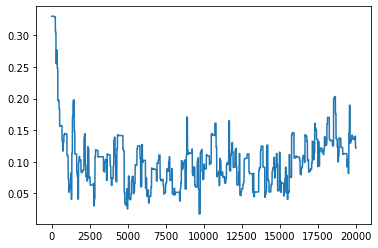
\includegraphics[width=0.45\textwidth]{conv1.png}} 
		\subfigure[]{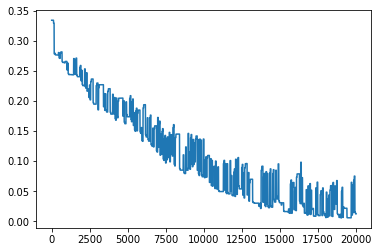
\includegraphics[width=0.45\textwidth]{conv2.png}} 
		\subfigure[]{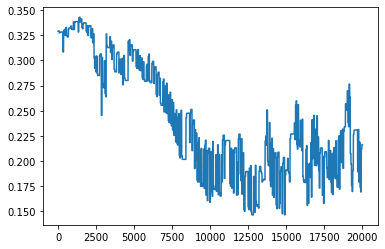
\includegraphics[width=0.45\textwidth]{conv3.png}}
		\subfigure[]{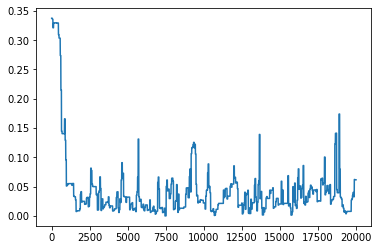
\includegraphics[width=0.45\textwidth]{conv4.png}}
		\caption{
			نمودار‌های مربوط به تغیرات معیار همگرایی وزن‌های اتصالات مابین جمعیت‌های لایه ۲/۳ یک ستون کورتکسی متصل به ورودی و جمعیت‌های حاضر در لایه ۴ ستون کورتکسی سوم.
			(آ) اتصالات بین دو جمعیت متناظر با الگوی اول.
			(ب) اتصالات بین جمعیت پیش‌سیناپسی متناظر با الگوی اول و جمعیت پس‌سیناپسی متناظر با الگوی دوم.
			(ج) اتصالات بین جمعیت پیش‌سیناپسی متناظر با الگوی دوم و جمعیت پس‌سیناپسی متناظر با الگوی اول. 
			(د) اتصالات بین دو جمعیت متناظر با الگوی دوم.
		}
		\label{fig:convergence}
	\end{figure}
	
	\subsection{بررسی وجود انقیاد در مدل}
	
	در مدل ارائه شده، فعالیت هم‌زمان دو ورودی مجزا، که هریک بیانگر یک ورودی سنسوری هستند، نهایتا پس از آموزش موجب فعالیت در ستون کورتکسی سوم می‌شوند که بیان‌گر یک مفهوم انتزاعی از چیزی است که دو ورودی سنسوری متعلق به آن هستند. در صورت رخ دادن انقیاد در مدل باید فعالیت حتی یکی از ورودی‌ها نیز باعث فعال شدن شبکه‌های عصبی متناظر با مفهوم کلی مورد نظر شوند که به عبارتی یعنی تنها در صورت فعالیت یکی از ورودی‌ها باید ما شاهد رفتار درست لایه ۲/۳ ستون کورتکسی سوم باشیم.
	
	برای بررسی این مورد یکی از جمعیت‌های ورودی را مشابه با زمان آموزش فعال می‌کنیم و جمعیت دیگر را بدون هیچ الگویی و تنها با مجموعه از فعالیت‌های تصادفی تعریف می‌کنیم و انتظار داریم در ستون کورتکسی سوم فعالیت مورد نظر را مشاهده کنیم. نمایش شطرنجی فعالیت مربوط به جمعیت‌های ورودی و جمعیت‌های لایه ۲/۳ ستون کورتکسی سوم در یک بازه‌ی زمانی ۴۰۰ میلی‌ثانیه‌ای در تصویر \ref{fig:binding-c1-c3} آورده شده است و کاملا مشهود است که انقیاد در این شبکه شکل گرفته است. هم‌چنین این موضوع به صورت برعکس ،یعنی به صورتی که جمعیت ورودی فعال در تصویر \ref{fig:binding-c1-c3} غیر فعال باشد و جمعیت دیگر فعال باشد، نیز بررسی قرار گرفته (تصویر \ref{fig:binding-c2-c3}) و صادق بودن این موضوع در آن صورت نیز مشخص شده است.
	
	\begin{figure}[H]
		\centering
		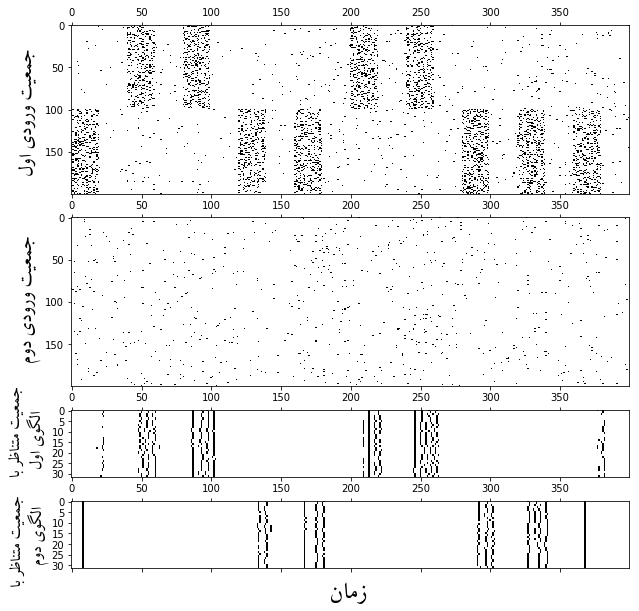
\includegraphics[width=1.0\linewidth]{binding-c1-c3.png}
		\caption[NS]{
			تصویر مربوط به بررسی وجود انقیاد در زمان نمایش الگو توسط جمعیت ورودی اول. در تصویر فوق سطر اول فعالیت جمعیت ورودی اول، سطر دوم جمعیت ورودی دوم و سطر سوم و چهارم نیز نشان دهنده‌ی فعالیت جمعیت‌های لایه‌ی ۲/۳ ستون کورتکسی سوم هستند.
		}
		\label{fig:binding-c1-c3} 
	\end{figure}

\begin{figure}[H]
	\centering
	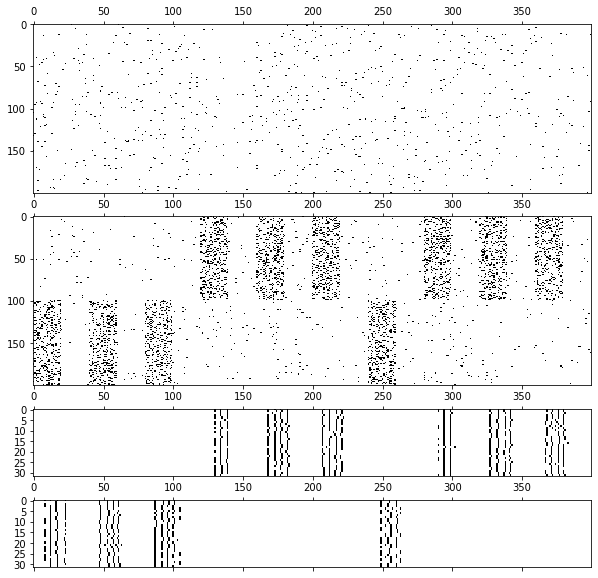
\includegraphics[width=1.0\linewidth]{binding-c2-c3.png}
	\caption[NS]{
		تصویر مربوط به بررسی وجود انقیاد در زمان نمایش الگو توسط جمعیت ورودی دوم. مشابه با تصویر \ref{fig:binding-c1-c3}، در این تصویر نیز سطر اول فعالیت جمعیت ورودی اول، سطر دوم جمعیت ورودی دوم و سطر سوم و چهارم نیز نشان دهنده‌ی فعالیت جمعیت‌های لایه‌ی ۲/۳ ستون کورتکسی سوم هستند.
	}
	\label{fig:binding-c2-c3} 
\end{figure}

	
	
	\chapter{جمع‌بندی و پیشنهاد کار‌های آینده}
	در این فصل به جمع‌بندی نهایی پژوهش انجام شده و مقایسه‌ی آن با فعالیت‌هایی خواهیم پرداخت که پیش از این برای توجیه و مدل‌سازی مسئله‌ی انقیاد انجام شده است. همچنین در نهایت به پژوهش‌هایی خواهیم پرداخت که می‌توان در ادامه‌ی این پژوهش به آن‌ها پرداخت.
	
	\section{مقایسه‌ی مدل ارائه شده با مدل‌های پیشین}
	چنان‌چه پیش از این نیز اشاره شد، در مدل‌های پیشین از روش‌های گوناگونی برای مدل‌سازی انقیاد استفاده شده است. اما حتی در نزدیکترین مدل ارائه شده در گذشته به ساختار‌های زیستی نیز فاصله‌ی قابل توجهی با واقعیت وجود داشت. در این پژوهش تلاش شده تا مدل ارائه شده از تمام جنبه‌ها یک مدل بسیار نزدیک به ساختار مغز باشد. چنانچه برای مدل‌سازی نورون‌ها از شبکه‌های عصبی ضربه‌ای استفاده شده که نزدیکترین مدل‌های نورونی به نورون‌های زیستی هستند و برای توپولوژی آن‌ها نیز تلاش شده از یک الگوی ارتباطی بسیار مشابه با ستون‌های کورتکسی حاضر در نئوکورتکس الگوبرداری شود تا از هر بابتی یک مدل نزدیک به ساختار زیستی باشد.
	
	این در حالی است که در تحقیقاتی که پیش از این صورت گرفته است، در بسیاری از موارد ساختار ارتباطی و نورون‌ها هیچ شباهتی به مدل‌های زیستی ندارند. همچون موارد استفاده از شبکه‌های عصبی رمزگذار-رمزگشای مولد که یک نمونه از همین موارد است.
	
	در این دسته از مدل‌سازی ها که هدف آن‌ها ارائه‌ی یک رویکرد و ساختار محاسباتی برای حل مسئله‌ی انقیاد است و در حال حاضر برای مسائلی همچون دسته‌بندی یا رگرسیون از آن‌ها استفاده نمی‌شود، برای مقایسه معیار عددی مشخصی نمی‌توان تعریف کرد ولی با توجه به هدف نهایی، که شکل دادن انقیاد است، و علم به رخ دادن انقیاد در مغز و اهمیت آن در ادراک مدل‌های مبتنی بر زیست در صورت نشان دادن عملکرد مناسب بسیار ارزشمند هستند.
	
	\section{نتیجه‌گیری}
	در این پژوهش نشان داده شد که ستون‌های کورتکسی توانایی پردازش اطلاعات و نهایتا شکل دادن انقیاد را دارند که یک عملکرد شناختی بسیار مهم و پیچیده در پستانداران است و این امکان وجود دارد که مشابه با انقیاد، ستون‌های کورتکسی توانایی تشکیل دادن بسیاری دیگر از عملکرد‌های شناختی را داشته باشند که یک گام به سوی ساختن عامل‌هایی با هوشمندی مشابه با موجودات زنده است.
	
	همچنین این ویژگی ستون‌های کورتکسی که ساختار و الگوی ارتباطی یکسانی دارند، باعث می‌شود تا بتوان از آن‌ها به سادگی به عنوان بلوک‌هایی تکرار شونده در شبکه‌های عصبی استفاده کرد و شبکه‌هایی ساخت که با از کنار هم قرار گرفتن مجموعه‌ای از ستون‌های کورتکسی، قادر به مدل‌سازی عملکرد‌های پیچیده‌ای هستند.
	
	\section{فعالیت‌های آینده}
	در این پژوهش هر لایه از ستون‌های کورتکسی به دو دسته تقسیم شده بود تا فرایند یادگیری و تفکیک فعالیت نورون‌های مقید شده به هر الگوی ورودی مشخص‌تر باشد. از جمله پژوهش‌هایی که می‌توان در ادامه‌ی این پژوهش انجام داد می‌توان به این مورد اشاره کرد که تعداد جمعیت‌‌های داخل هر لایه افزایش یابد تا بتواند تفکیک را بین بیش از دو الگو نیز با استفاده از ستون‌های کورتکسی انجام داد. همچنین می‌توان بجای در نظر گرفتن تعداد مشخصی جمعیت، هر لایه را یک جمعیت یک‌پارچه در نظر گرفت و انتظار داشت در طول آموزش، هر نورون به مرور زمان به یکی از الگو‌های ورودی مقید شود که  مدلی بسیار نزدیکتر به ساختار زیستی مغز و ستون‌های کورتکسی حاضر در مغز است.

	
	
	
	%#######################################################
	%#######################################################
	%#######################################################
	%#######################################################
	
	
	
	%Glossaries-----------------------------------
	
	\printglossary[title=واژه‌نامه فارسی به انگلیسی, toctitle=واژه‌نامه فارسی به انگلیسی]
	
	%References-----------------------------------
	
	%\begin{thebibliography}{MM}
	\begin{latin}
		\bibliographystyle{abbrv}
		\renewcommand{\bibname}{\rl{{مراجع}\hfill}}
		%	\addcontentsline{toc}{chapter}{کتاب‌نامه}
		\bibliography{references}
	\end{latin}
	%\end{thebibliography}
	
	%Abstract En----------------------------------
	\linespread{1}
	\begin{latin}
		\begin{abstract}
			Binding problem is one of the important problems in neuroscience, cognitive sciences and philosophy of mind. It's about how a living organism's understanding is integrated from partial concepts formed in the brain. The importance of this problem is in understanding of human cognitive functions, which itself is part of steps required to designing systems that are capable of processing cognitive functions that are similar to humans. Researches show the very strong role of cortical columns, which are structures in the neocortex, in the cognitive functions of living organisms. In this research, an attempt has been made to simulate the formation of binding in the brain by modeling the cortical columns and the relationships between them using spiking neural networks. Finally, the tests and investigations carried out on the designed model show the formation of binding in the presented model. This issue indicates that probably the cortical columns, as defined structures that can be easily replicated in modeling, are potentially suitable structures to be used in modeling and increase the possibility of forming cognitive processes in the model.
			
			\section*{}
			\textbf{Keywords:}\quad Cortical Column, Binding Problem, Spiking Neural Network, Modeling.
		\end{abstract}
		\newpage
		
		%Title page En -------------------------------
		\begin{figure}
			\centering
			
\includegraphics[height=2.5cm]{ut.png}
		\end{figure}
		\begin{center}
			
			College of Science\\
			School of Mathematics, Statistics, and Computer Science
		\end{center}
		
		\begin{center}
			%%%%%%%%%%%%%
		\end{center}
		
		\begin{center}
			\huge{Modeling the Mechanisms of Binding Problem in Spiking Neural Networks}
		\end{center}
		
		\begin{center}
			%%%
		\end{center}
		
		\begin{center}
			\textbf{
				Amir Aslan Aslani
				\\[30pt]
			}
		\end{center}
		
		
		\begin{center}
			Supervisors
		\end{center}
		\begin{center}
			\textbf{
				Mohammad Ganjtabesh
				\\[5pt]
				Abbas Nouzari Dalini
			}
		\end{center}
		
		
		\vspace{3cm}
		\begin{center}
			A thesis submitted to Graduate Studies Office\\
			in partial fulfillment of the requirements for the degree of \\
			Master of Science in\\
			Computer Science
		\end{center}
		
		\begin{center}
			February 2022
		\end{center}
		
		%\pagestyle{empty}
		%\pagenumbering{}
		
	\end{latin}
	
\end{document}
%####################################################################
%########### END DOCUMENT ###########################################
%####################################################################